% Plantilla realizada por Alberto Brunete (UPM).

%Parametros de tipo libro
\documentclass[10pt,a4paper]{book}

%Idioma español y acentos
%\usepackage[spanish, es-tabla]{babel}
%\usepackage[latin1]{inputenc}
\usepackage[utf8]{inputenc}

%algunos sÌmbolos matemáticos y paquetes para usar subimágenes
\usepackage{amsmath}
\usepackage{amsfonts}
\usepackage{amssymb}
\usepackage{graphicx}
\usepackage{subfigure}
\usepackage{listings}
\usepackage{appendix}
\usepackage{array}
\usepackage{multirow} 
\usepackage{pgfgantt}
\usepackage{xcolor}
%Márgenes
\usepackage[left=3cm,top=3cm,right=3cm,bottom=3cm]{geometry}

%
\usepackage{multicol}

%para generar índice con hipervínculos
\usepackage{hyperref}

%parametros del documento (sus propiedades)
\hypersetup{
    pdftitle={Hugo de la Quintana Béjar - TFM - 2021},
    pdfsubject={TFM - 2021},
    pdfauthor={Hugo de la Quintana Béjar},
    pdfkeywords={Domótica} {palabraclave2} {palabraclave3},
    colorlinks,
    citecolor=black,
    filecolor=black,
    linkcolor=black,
    urlcolor=black,
}

%Código
\usepackage{listings}
%Rename Listlings
\renewcommand{\lstlistingname}{Código}% Listing -> Algorithm
\renewcommand{\lstlistlistingname}{Lista de \lstlistingname s}
% List of Listings -> Lista de Código

%empieza el documento
\begin{document}  

%elementos antes del trabajo en sÌ se meten dentro de frontmatter
\frontmatter

%cada incluye referencia a un archivo de tipo .tex
\begin{titlepage}
\begin{center}

%forma de introducir imágenes. el \\[0.5 cm] de final de línea introduce un salto de ese tamaño.
%width=1\textwidth indica el tamaño de la imágen (valores entre 0-1). 
 
\includegraphics[width=1\textwidth]{figures/cabecera.png}  \\[0.75 cm]

\LARGE UNIVERSIDAD POLITÉCNICA DE MADRID \\ [1 cm]

\LARGE ESCUELA TÉCNICA SUPERIOR DE INGENIEROS INDUSTRIALES \\ [1 cm]

\LARGE Máster en Automática y Robótica\\ [1 cm]

\LARGE \textbf{TRABAJO FIN DE MASTER}\\[1 cm]

\Huge \textsc{Planificación y Diseño de una Instalación Domótica Real mediante el uso del Protocolo KNX}\\[1 cm]

\LARGE Hugo de la Quintana Béjar \\[2 cm]

%flushleft alinea a la izquierda el texto

 \Large 
\emph{Tutor:} Alberto Brunete González\\
\emph{Departamento:} Ingeniería Eléctrica, Electrónica \\
\emph{} Automática y Física Aplicada


%rellena de blanco el resto de la página para escribir abajo del todo
\vfill

% Bottom of the page
{\large Madid, Julio, 2021}

%SE ponen al final firmas.tex
%\end{center}
%\end{titlepage}


\cleardoublepage 


%\begin{center}
% Está puesto en portada.tex
\thispagestyle{empty}
%forma de introducir imágenes. el \\[0.5 cm] de final de línea introduce un salto de ese tamaño.
%width=1\textwidth indica el tamaño de la imágen (valores entre 0-1). 

\includegraphics[width=1\textwidth]{figures/cabecera.png}  \\[0.5 cm]

\LARGE UNIVERSIDAD POLITÉCNICA DE MADRID \\ [1 cm]

\LARGE ESCUELA TÉCNICA SUPERIOR DE INGENIEROS INDUSTRIALESL \\ [1 cm]

\LARGE Máster en Automática y Robótica\\ [1 cm]

\LARGE \textbf{TRABAJO FIN DE MASTER}\\[1 cm]

\Huge \textsc{Planificación y Diseño de una Instalación Domótica Real mediante el uso del Protocolo KNX}\\[3 cm]

%flushleft alinea a la izquierda el texto

\begin{multicols}{2} 
\begin{flushleft} 
\Large \emph{Firma Autor}
\end{flushleft}

\begin{flushright} 
\Large \emph{Firma Tutor}
\end{flushright}

\end{multicols} 

%rellena de blanco el resto de la página para escribir abajo del todo
\vfill

\end{center}
\end{titlepage}


\cleardoublepage 

%Licencia opcional
\begin{flushleft}

Copyright \copyright  año. Nombre del alumno

%ejemplo de licencia, se puede elegir cualquier otra

Esta obra está licenciada bajo la licencia Creative Commons Atribución-NoComercial-SinDerivadas 3.0 Unported (CC BY-NC-ND 3.0). Para ver una copia de esta licencia, visite http://creativecommons.org/licenses/by-nc-nd/3.0/deed.es o envíe una carta a Creative Commons, 444 Castro Street, Suite 900, Mountain View, California, 94041, EE.UU.

Todas las opiniones aquí expresadas son del autor, y no reflejan necesariamente las opiniones
de la Universidad Politécnica de Madrid.

\end{flushleft}

\cleardoublepage

\begin{flushleft} \large
\textbf{Título:}Planificación y Diseño de una Instalación Domótica Real mediante el uso del Protocolo KNX \\
\textbf{Autor:} Hugo de la Quintana Béjar\\
\textbf{Tutor:} Alberto Brunete González \\ 

\end{flushleft} 

\begin{center} \LARGE
EL TRIBUNAL \\ [1 cm]
\end{center}

\begin{flushleft} \LARGE
Presidente: \\ [1 cm]
Vocal: \\ [1 cm]
Secretario: \\ [1.5 cm]
\end{flushleft}

\large
Realizado el acto de defensa y lectura del Trabajo Fin de Grado el día ....... de ....................   de ... en .........., en la Escuela Técnica Superior de Ingeniería y Diseño Industrial de la Universidad Politécnica de Madrid, acuerda otorgarle la CALIFICACIÓN de: \\ [2 cm]

\begin{center}
 \large VOCAL \\ [2.2 cm]
\end{center}

\begin{minipage}{0.5\textwidth}
 \begin{flushleft}
 \large SECRETARIO
\end{flushleft}
\end{minipage}
\begin{minipage}{0.5\textwidth}
\begin{flushright}
 \large PRESIDENTE
\end{flushright} 
\end{minipage}

\chapter{Acknowledgements}

Agradezco a ............

%chapter introduce un nuevo capítulo

\chapter{Resumen}

El presente trabajo fue llevado a cabo con la supervisión y la financiación de la empresa Freedom Ingeniería y Domótica, ubicada en la ciudad de Madrid, España, enmarcada en el sector de las instalaciones eléctricas, las telecomunicaciones y el diseño de sistemas domotizados. \\
Con el fin de lograr el mejor resultado en este proyecto, la empresa pondrá a disposición del autor todos los recursos necesarios para su correcto desarrollo, siempre dentro de los marcos económicos y temporales posibles de otorgar a un proyecto de estas características.\\
 El objetivo del TFM es planificar y diseñar una instalación domótica real en una residencia, así como realizar su puesta en marcha. En cuanto a las funcionalidades a implementar, se considera el control del sistema de iluminación y persianas, implementación y programación de pantallas, control de consumos, control sensorial, fusión de sistemas para el control de la climatización, protocolos de comunicación local y remota. Otros objetivos serían optimizar el diseño de la instalación para ajustarse al máximo rendimiento y ahorro energético, y establecer un sistema de contadores para realizar un sistema de control de consumo de recursos (energía, agua). \\\\
Para lograr alcanzar esos objetivos de manera óptima, se plantearán diversas fases del proyecto en el que estarán marcados una serie de hitos para facilitar así el control de la evolución del mismo, como pueden ser la consecución del software y material necesarios o partes del desarrollo de las programaciones de los mecanismos a implementar.\\\\
Todo ello se deberá definir y concretar con un cliente y unos proveedores reales, atendiendo a sus peticiones y requisitos, por lo que también serán necesarias aptitudes comunicativas y de negociación a la hora de lograr llegar a acuerdos en los puntos en los que sea necesaria su intervención.

\paragraph{Keywords:} tecnología, control, domótica.


\chapter{Abstract}

The present work was carried out with the supervision and financing of Freedom Ingeniería y Domótica, a company based in Madrid, Spain, dedicated to electrical installations, telecommunications and the design of home automation systems. \\
As a means to achieve the best result, the company has provided the author with all necessary resources for the development of this project, within the usual budgetary and temporary frames for a design of these characteristics.\\
The purpose of the thesis is to design, plan and implement a real home automation installation. Regarding the functionality requirements, it features the lightning system control, blind controls, consumption control, sensory control, a merging of systems for climate control, and also local and remote communication protocols as well as the implementation and programming of screens. Other objectives would be to optimize the design of the installation so as to get the highest performance and energy saving; and to set up a meter system to be able to control the consumption of resources (energy, water). \\\\
In order to achieve these objectives, the project is conducted in different phases. Milestones have been set in each phase to ease the control of the evolution of the project, such as the acquisition of the needed software, or the different programming stages of the implemented mechanisms. \\\\
Also, all of that must be defined along with the real customer and suppliers, according to their requests and requirements. Therefore, communication and negotiation skills will also be necessary to reach agreements on the points where their intervention is necessary.


\paragraph{Keywords:} technology, control, home automation.

%genera índice
\tableofcontents
\addcontentsline{toc}{chapter}{Índice}

%Índice de figuras.
\listoffigures

%Índice de tablas.
\listoftables

%Empieza la parte descriptiva del trabajo
\mainmatter

\chapter{Introducción}

Como pequeña introducción, es importante señalar que todo lo que aparezca en la memoria debe ser original. Si aparecen textos de otros libros, artículos o webs, deben ir convenientemente referencidos.

En este capítulo no deben faltar los siguientes apartados:

\section{Motivación}

Motivación o Marco del proyecto, es donde se cuenta cómo surgió la idea del proyecto y se da un breve resumen explicativo.

\section{Objetivos y campos de aplicación}

Es muy importante señalar el objetivo principal del TFG, así como los objetivos secundarios que se estableciaron al principio o han ido surgiendo durante su elaboración.

\section{Structure of the document}

A continuación y para facilitar la lectura del documento, se detalla el contenido de cada capítulo.

\begin{itemize}
\item En el capítulo 1 se realiza una introducción.
\item En el capítulo 2 se hace un repaso...
\end{itemize}

  
  %partes finales del trabajo: conclusiones, bibliografia y anexos

\chapter{Conceptos teóricos}

En este capítulo se describen (brevemente) todos los conceptos necesarios para entender el trabajo. No se trata de copiar el contenido de los libros de texto, si no de hacer un resumen de los conceptos necesarios para facilitar la lectura del documento al lector. Se entiende que el lector de un TFG tiene que tener unos conocimientos mínimos sobre el tema.

\section{¿Qué es la domótica?}

mimi

\section{Marco histórico}

mimi

\section{¿Qué es KNX?}

knx, protocolos, teoria clase...)

\section{Lista de materiales}

A continuación, se detalla una lista con los múltiples dispositivos y módulos domóticos que han sido utilizados para desarrollar la solución final diseñada y la funcionalidad que les ha sido otorgada. En esta lista únicamente aparecerán los elementos incluidos en el cuadro eléctrico de domótica y los mecanismos domóticos de la instalación, quedando excluidos, por tanto, los efectores y actuadores puramente eléctricos así como su cuadro, por no encontrarse dentro de las competencias de diseño del sistema.

\subsection{\textbf{Actuadores:}} Estos elementos se encargan de ejecutar las acciones solicitadas desde el controlador sobre los diferentes elementos domóticos de la vivienda a los que se encuentra conectado. Existen diversas clases de actuadores que se clasifican en función de la aplicación que vayan a desarrollar. En este proyecto se utilizarán los siguientes:

\begin{itemize}
\item \textbf{Dimmers:} 
	\begin{itemize}
	\item\underline{Descripción:} actuador regulador KNX de 4 elementos.
	\item \underline{Características:} este tipo de actuador permite el control de la regulación del elemento que se encuentra conectado a su salida mediante el uso de dispositivos TRIAC y DIAC. Cuenta con modo de accionamiento manual para modo de prueba, además de protección contra marcha en vacío, cortocircuito y sobretemperatura. 
	\item \underline{Funcionalidad:} la aplicación que ejecutan es la de regulación de la intensidad de la iluminación de algunas de las lámparas de la vivienda.\\ [0,15 cm]
		\begin{figure}[h]
		\centering
		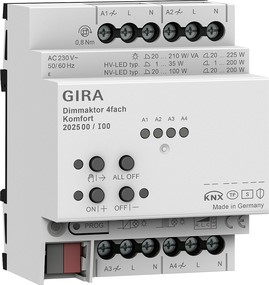
\includegraphics[width=0.35\textwidth]{figures/actuador_dimmer.jpg}   
		\caption{Actuador tipo dimmer}
		\label{fig:actuador_dimmer}
		\end{figure}
	\end{itemize} 


\item \textbf{Binario + persiana:} 
	\begin{itemize}
	\item\underline{Descripción:} actuador de conmutación de 24 elementos / control 12 persianas.
	\item \underline{Características:} este módulo combina la funcionalidad de dos tipos de actuadores diferentes, y permite el control tanto de elementos ON/OFF como de persianas, atendiendo a la funcionalidad con la que se programen sus salidas. Cuenta con modo de accionamiento manual para modo de prueba.
	\item \underline{Funcionalidad:} algunas de sus salidas serán utilizadas para el control de apertura de una ventana y el despliegue de una pantalla de proyección. El resto servirán para el control binario del resto de luces de la casa y de algunas de las tomas de corriente que se han decidido “domotizar”. Otras funcionalidades puntuales de tipo binario que tienen sus salidas son las de accionamiento del timbre, de la sirena de alarma, el control de la cerradura de la vivienda, la velocidad del recuperador, el encendido de la caldera y las electroválvulas de agua y gas.
	\begin{figure}[h]
	\centering
	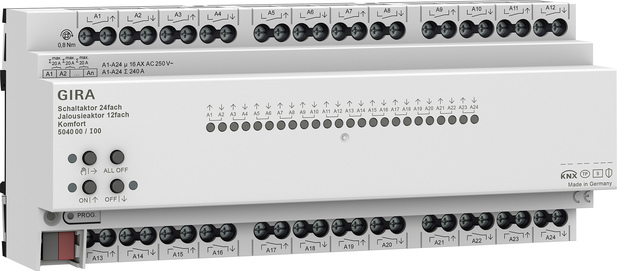
\includegraphics[width=0.55\textwidth]{figures/actuador_binario.png}   
	\caption{Actuador tipo binario/persiana}
	\label{fig:actuador_binario}
	\end{figure}
	\end{itemize} 

\item \textbf{Rejilla + zonificación:} 
	\begin{itemize}
	\item\underline{Descripción:} actuador de control sobre 8 rejillas + 2 unidades de aire acondicionado.
	\item \underline{Características:} esta clase de actuador combina la capacidad de control de la apertura de una rejilla con la de gestión de diferentes temperaturas mediante módulos lógicos. . Cuenta con modo de accionamiento manual para modo de prueba, además de indicadores visuales de movimiento de rejillas mediante LEDs.
	\item \underline{Funcionalidad:} gracias a sus características, nos permite conectarlo con los termostatos distribuidos por la casa y hacer un control por zonas de la distribución del sistema de aerotermia de los fancoils, activando y adecuando la velocidad de sus ventiladores en función de la demanda.
	\begin{figure}[h]
	\centering
	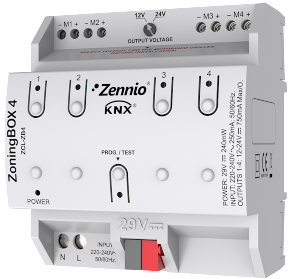
\includegraphics[width=0.35\textwidth]{figures/actuador_rejilla.png}   
	\caption{Actuador tipo zonificación}
	\label{fig:actuador_rejilla}
	\end{figure}
	\end{itemize} 

\item \textbf{Accionamiento térmico:} 
	\begin{itemize}
	\item\underline{Descripción:} actuador de calefacción de 6 elementos.
	\item \underline{Características:} permite la actuación de accionamientos térmicos integrado con un regulador de temperatura ambiente. Incluye la opción del conexionado en cascada de los actuadores.
	\item \underline{Funcionalidad:} las salidas de este módulo irán conectadas a las válvulas de regulación de los entramados del suelo radiante para regular su apertura, así como a la caldera de la vivienda, indicando los momentos en los que esta debe ser activada en función de la demanda de temperatura gestionada por los termostatos. \\ [0,15 cm]
	\begin{figure}[h]
	\centering
	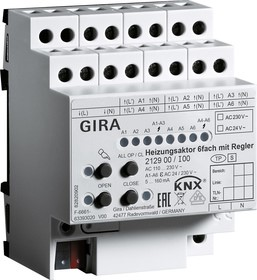
\includegraphics[width=0.35\textwidth]{figures/actuador_termico.jpg}   
	\caption{Actuador tipo térmico}
	\label{fig:actuador_termico}
	\end{figure}
	\end{itemize} 
\end{itemize} 

\subsection{\textbf{Sensores}}

\begin{itemize}
\item \textbf{CO\textsubscript{2}:} 
	\begin{itemize}
	\item\underline{Descripción:} sensor CO\textsubscript{2} con regulador de humedad y temperatura KNX.
	\item \underline{Características:} supervisión del valor de partículas de \textsubscript{2} y de humedad en el ambiente. Alarma de punto de rocío para prevenir la formación de moho en sistemas de refrigeración. Posee dos entradas binarias para la conexión de contactos sin tensión. El sensor de \textsubscript{2} permite ajustar cuatro niveles límites diferentes.
	\item \underline{Funcionalidad:} la funcionalidad con la que ha sido programado es la de, mediante la actuación de tres niveles de partículas de \textsubscript{2}, activar los tres niveles de velocidad del ventilador del recuperador en consecuencia.
	\begin{figure}[h]
	\centering
	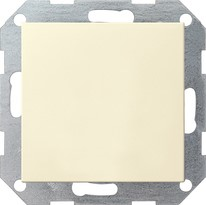
\includegraphics[width=0.30\textwidth]{figures/sensor_co2.jpg}   
	\caption{Sensor de CO\textsubscript{2}}
	\label{fig:sensor_co2}
	\end{figure}
	\end{itemize} 


\item \textbf{Movimiento:} 
	\begin{itemize}
	\item\underline{Descripción:} detector de movimiento de superficie de 2,2 m.
	\item \underline{Características:} configurable para la detección de movimiento o para la monitorización del con capacidad de cuantificar la luminosidad de la estancia para realizar un apagado de la iluminación al superar un umbral configurable. Permite la configuración de un bloque de función para realizar las siguientes funciones: conmutación, función para escaleras, transmisor de valores de regulación, mecanismo auxiliar para escenarios, transmisor de valores de temperatura, transmisor de valores de luminosidad, conmutación de modo de funcionamiento, conmutación con posición forzada.
	\item \underline{Funcionalidad:} serán utilizados para detectar la entrada de personas en determinadas zonas de la vivienda, y en función del modo en que se encuentre el sistema, hará las veces de ON/OFF de las luces de esas zonas o bien hará saltar el sistema de alarma ante intrusiones.
	\begin{figure}[h]
	\centering
	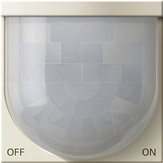
\includegraphics[width=0.25\textwidth]{figures/sensor_movimiento.png}   
	\caption{Sensor de movimiento}
	\label{fig:sensor_movimiento}
	\end{figure}
	\end{itemize} 

\item \textbf{Presencia:} 
	\begin{itemize}
	\item\underline{Descripción:} detector presencia multifunción.
	\item \underline{Características:} posee varios modos de funcionamiento, a saber: detector de presencia, observador de techo o detector de movimiento. La monitorización del entorno se realiza mediante el uso de tres sensores PIR y uno de luminosidad, con lo que se permite utilizar los parámetros de detección de las tres zonas y de luminosidad para hacer un control en intensidad de la iluminación zonal en sintonía con la posibilidad de utilizar las cinco funciones lógicas que permite usar. La funcionalidad de este dispositivo es similar a la del detector de movimiento, pero con los siguientes añadidos: transmisión de valores de regulación, nivel crepuscular ajustable, aplicación de retardos, función de bloqueo y la posibilidad de configuración de límites de luminosidad.
	\item \underline{Funcionalidad:} gracias a su diseño discreto, se instala en el techo del salón con la funcionalidad de controlar la iluminación de la estancia en función de principalmente dos parámetros externos: la presencia de personas y la iluminación exterior, aplicándole un valor de sensibilidad determinado para realizar el ON a partir de la detección de cierta cantidad de luxes.
	\begin{figure}[h]
	\centering
	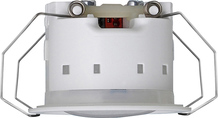
\includegraphics[width=0.35\textwidth]{figures/sensor_presencia.png}   
	\caption{Sensor de presencia}
	\label{fig:sensor_presencia}
	\end{figure}
	\end{itemize}

\item \textbf{Inundación:} 
	\begin{itemize}
	\item\underline{Descripción:} sensor de inundación.
	\item \underline{Características:} es capaz de detectar la presencia de agua en un ambiente.
	\item \underline{Funcionalidad:} será necesario la implementación de un módulo de entradas para poder comunicar los sensores con la instalación KNX de la vivienda.
	\begin{figure}[h]
	\centering
	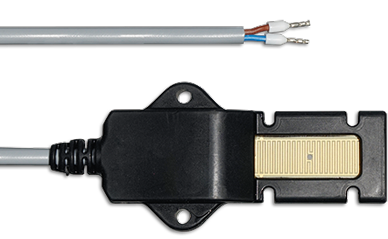
\includegraphics[width=0.35\textwidth]{figures/sensor_inundacion.png}   
	\caption{Sensor de inundación}
	\label{fig:sensor_inundacion}
	\end{figure}
	\end{itemize} 

\item \textbf{Apertura:} 
	\begin{itemize}
	\item\underline{Descripción:} contacto magnético.
	\item \underline{Características:} este sensor consta de dos partes: la primera irá fijada en el marco de la ventana y la segunda, en la propia ventana. Al cerrar la ventana, se cerrará el circuito eléctrico, transmitiendo así un valor por el bus opuesto al que envía al encontrarse abierto.
	\item \underline{Funcionalidad:} su misión será la de ofrecer al sistema información acerca de si las ventanas de la casa se encuentran abiertas o cerradas.
	\begin{figure}[h]
	\centering
	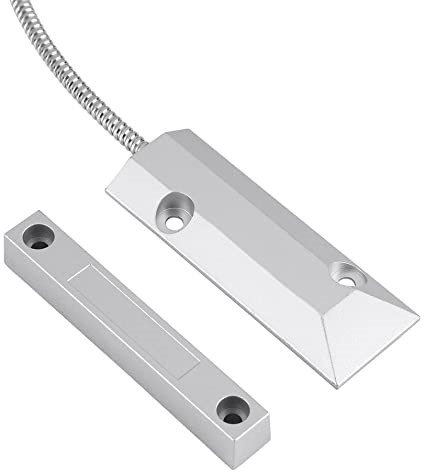
\includegraphics[width=0.35\textwidth]{figures/sensor_apertura.png}   
	\caption{Sensor de apertura}
	\label{fig:sensor_apertura}
	\end{figure}
	\end{itemize} 

\item \textbf{Humo:} 
	\begin{itemize}
	\item\underline{Descripción:} combinación de detector de humos y detector térmico.
	\item \underline{Características:} sensor termovelocimétrico alimentado por pilas. Dos señales acústicas de alarma distintas para cada uno tipos de detección con posibilidad de atenuarse durante la fase de pruebas.
	\item \underline{Funcionalidad:} su objetivo es el de detectar de situaciones anómalas y potencialmente peligrosas relacionadas con los incendios y dar aviso de ello a los usuarios que se encuentren en la vivienda. Para poder ser integrados en la instalación KNX, será necesario la implementación de un módulo extra, que será el encargado de comunicar el detector de humos con el sistema de control de la vivienda.
	\begin{figure}[h]
	\centering
	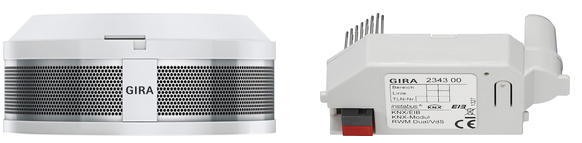
\includegraphics[width=0.75\textwidth]{figures/sensor_humo.png}   
	\caption{Sensor de humo y módulo KNX}
	\label{fig:sensor_humo}
	\end{figure}
	\end{itemize} 
\end{itemize} 

\subsection{\textbf{Lectores de consumo}}

\begin{itemize}
\item \textbf{Electricidad:} 
	\begin{itemize}
	\item\underline{Descripción:} medidor de energía eléctrica para sistemas monofásicos o trifásicos.
	\item \underline{Características:} permite el monitorizar la energía consumida/producida, el coste y las emisiones de \textsubscript{2} asociadas al consumo, la potencia activa y reactiva, el factor de potencia y otra información relacionada con el uso de la energía en la vivienda.
	\item \underline{Funcionalidad:} se monitorizarán la tensión y corriente de fase instantáneos, la potencia activa consumida instantánea y la energía consumida acumulada total y en un periodo de tiempo definido por el usuario, incluyendo la tarifa y sus emisiones de carbono en esos periplos. Se realizarán dichas medidas acoplando un transformador de corriente a cada una de las líneas. 
	\begin{figure}[h]
	\centering
	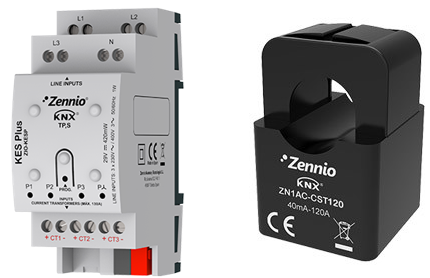
\includegraphics[width=0.55\textwidth]{figures/contador_electricidad.png}   
	\caption{Contador consumo eléctrico y acoplador de línea }
	\label{fig:contador_electricidad}
	\end{figure}
	\end{itemize} 

\item \textbf{Agua y gas:} 
	\begin{itemize}
	\item\underline{Descripción:} interfaz KNX de monitorización de consumo de 4 elementos.
	\item \underline{Características:} permite monitorizar en el bus KNX el consumo eléctrico (energía y potencia), agua y gas mediante el conteo de pulsos SO (salida impulso optoacoplador). Estas medidas pueden visualizarse en consumo instantáneo o acumulado.
	\item \underline{Funcionalidad:} estos módulos serán utilizados para hacer un conteo del consumo acumulado total y desdeuna fecha determinada por el usuario del agua y el gas gastados en la vivienda. Tambien se utilizará su funcionalidad de calculo de tarifas, para que el cliente pueda consultar el gasto en cualquier periplo. Irá conectado directamente a los instrumentos de medida de la vivienda.
	\begin{figure}[h]
	\centering
	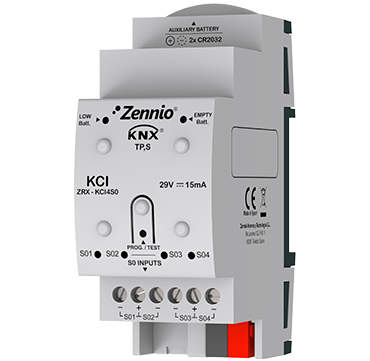
\includegraphics[width=0.35\textwidth]{figures/contador_agua.png}   
	\caption{Contador de consumo de agua y gas}
	\label{fig:contador_agua}
	\end{figure}
	\end{itemize} 
\end{itemize} 

\subsection{\textbf{Interfaces del usuario}}

\begin{itemize}
\item \textbf{Pulsadores domóticos:} 
	\begin{itemize}
	\item\underline{Descripción:} mecanismo acoplador de bus.
	\item \underline{Características:} de la variedad de características que pueden presentar este tipo de elementos, se han escogido los acopladores de bus con pulsación sobre dos elementos con mando de un punto, es decir, pulsadores de dos teclas con posibilidad de pulsarse únicamente en una dirección. 
	\item \underline{Funcionalidad:} control de las lámparas, tanto las binarias como las dimmeables, los enchufes, activación de las velocidades del recuperador, subir y bajar la pantalla del proyector, abrir y cerrar la ventana y activación del timbre.
	\begin{figure}[h]
	\centering
	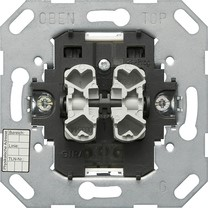
\includegraphics[width=0.30\textwidth]{figures/pulsador.jpg}   
	\caption{Pulsadores domóticos}
	\label{fig:pulsador}
	\end{figure}
	\end{itemize} 

\item \textbf{Termostatos:} 
	\begin{itemize}
	\item\underline{Descripción:} panel táctil capacitivo con display.
	\item \underline{Características:} posee 4 botones con multidisplay de 4 indicadores personalizables. Incluye funcionalidad de termostato, detector de movimiento y 2 puertos de entradas de tipo binario o lectura desde una sonda de temperatura.
	\item \underline{Funcionalidad:} se utilizará su función de termostato para gestionar el sistema de climatización. Desde estos dispositivos se efectuarán las llamadas de demanda tanto al sistema de suelo radiante como a los fancoils, en función de las temperaturas sensadas en cada habitación mediante el uso de una de sus entradas como sonda de temperatura. Uno de los termostatos llevará en su segunda canal de entrada una sonda térmica utilizada para conocer la temperatura exterior a la vivienda. Además, sus botones serán utilizados para las siguientes funciones:
		\begin{itemize}
		\item Los botones en el cuadrante inferior serán utilizados para subir y bajar la temperatura de consigna de la zona en la que se encuentra el termostato.
		\item El botón en el cuadrante superior derecho tendrá la funcionalidad de variar el flujo de aire cedido por los equipos de aire acondicionado. Al ser un único botón, la secuencia que efectuará será cíclica siguiente patrón: +, ++, +++, A, +. ++, +++, A, … Siendo A la ejecución del modo automático, que seleccionará la velocidad de los ventiladores en función de la demanda y la ponderación otorgada a cada zona o habitación.
		\item El botón en el cuadrante superior izquierdo servirá para cerrar la rejilla de esa habitación, evitando así el paso del aire de los fancoils.
		\end{itemize} 
	\begin{figure}[h]
	\centering
	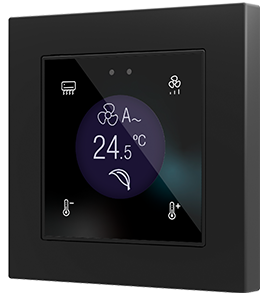
\includegraphics[width=0.37\textwidth]{figures/termostato.png}   
	\caption{Termostato}
	\label{fig:termostato}
	\end{figure}
	\end{itemize} 

\item \textbf{G1:} 
	\begin{itemize}
	\item\underline{Descripción:} es un dispositivo multifunción que permite visualizar y controlar numerosas funciones del edificio relacionadas con el control de los módulos instalados en ellos.
	\item \underline{Características:} posee una infinidad de funcionalidades, por lo que se mencionan únicamente las que poseen un enfoque más focalizado hacia las buscadas en este proyecto: una pantalla táctil con altavoz y micrófono integrados, capacidad de reconocimiento facial y reproducción de vídeo. Es posible personalizar su interfaz de usuario con la posibilidad de utilizar más de 320 iconos de función organizadas por carpetas con un manejo muy intuitivo. 
	\item \underline{Funcionalidad:} será utilizado como monitor y como puesto de control principal de la vivienda, representando la programación volcada sobre el X1. Esta pantalla hará las veces de display para mostrar las cadenas de texto o los datos que puedan resultar de interés para el usuario, como pudieran ser mensajes de alarma, de consumo, de avería o error... 
	\begin{figure}[h]
	\centering
	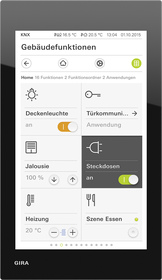
\includegraphics[width=0.25\textwidth]{figures/g1.png}   
	\caption{G1}
	\label{fig:g1}
	\end{figure}
	\end{itemize} 
\end{itemize} 

\subsection{\textbf{Módulos de entradas}}

\begin{itemize}
\item \textbf{Para sensores de apertura:} 
	\begin{itemize}
	\item\underline{Descripción:} entrada binaria KNX de 6 elementos.
	\item \underline{Características:} este módulo posee 6 entradas binarias que transforman sus valores en telegramas KNX. Permite ejecutar dos acciones diferentes por cada flanco, tanto de subida como de bajada, de cada una de las salidas.
	\item \underline{Funcionalidad:} en este proyecto, este mecanismo tendrá como entradas una serie de contactores magnéticos, cuya tarea es la de sensar el estado de las ventanas (abierto o cerrado), para que, en caso de pasar una cantidad de tiempo determinada en estado abierto, desconecte el sistema de climatización para esa estancia.
	\begin{figure}[h]
	\centering
	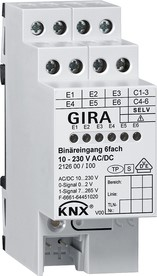
\includegraphics[width=0.2\textwidth]{figures/entradas_apertura.jpg}   
	\caption{Módulo 6 entradas para sensores de apertura}
	\label{fig:entradas_apertura}
	\end{figure}
	\end{itemize} 
\end{itemize} 

\subsection{\textbf{Pasarelas}}

\begin{itemize}
\item \textbf{Para sistema de aerotermia:} 
	\begin{itemize}
	\item\underline{Descripción:} pasarela Daikin –KNX.
	\item \underline{Características:} permite la comunicación bidireccional entre los sistemas Daikin VRV y las instalaciones KNX. 
	\item \underline{Funcionalidad:} su principal misión será la de servir de puente de comunicación entre el sistema propio de los sistemas de fancoil de la vivienda y el sistema domótico KNX, permitiendo así su control a través del bus mediante el envío de telegramas y su decodificación.
	\begin{figure}[h]
	\centering
	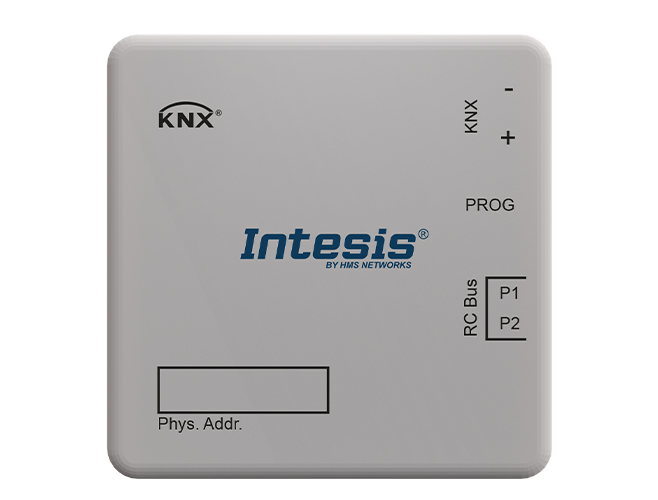
\includegraphics[width=0.47\textwidth]{figures/pasarela.png}   
	\caption{Pasarela para sistema de aerotermia}
	\label{fig:pasarela}
	\end{figure}
	\end{itemize} 
\end{itemize} 

\subsection{\textbf{Servidores}}

\begin{itemize}
\item \textbf{X1:} 
	\begin{itemize}
	\item\underline{Descripción:} servidor de visualización para terminales móviles.
	\item \underline{Características:}  este mecanismo permite la visualización de una interfaz personalizada en tu móvil o tablet  a través de internet, así como el control de hasta 250 funciones mediante el uso de comandos de voz o bien mediante la aplicación. Capacidad de uso de hasta 250 temporizadores, 36 bloques lógicos diferentes y 1450 datapoints.
	\item \underline{Funcionalidad:} contendrá los módulos lógicos programados para desarrollar las funcionalidades especiales del resto de módulos y el software sobre el que se programa la interfaz de visualización tanto del G1 como de la aplicación móvil. También permitirá la conexión remota a través de la aplicación móvil al alojar un servidor propio a través de la conexión Wi-Fi de la vivienda.
	\begin{figure}[h]
	\centering
	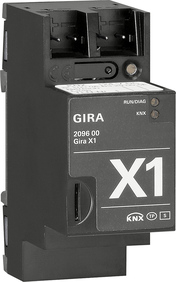
\includegraphics[width=0.23\textwidth]{figures/x1.png}   
	\caption{X1}
	\label{fig:x1}
	\end{figure}
	\end{itemize} 
\end{itemize} 

\subsection{\textbf{Fuentes de alimentación}}

Esta función será desarrollada por un módulo único compartido por ambos cuadros domóticos de la vivienda. Su cometido es el de transformar la corriente alterna proveniente de la acometida pública que llega a las casas con una tensión de 230V entre fase y neutro, en corriente continua de 29V, que es el potencial de bus necesario para alimentar los dispositivos. Este dispositivo no cuenta con ningún tipo de distribuidor de intensidad, por lo que la corriente nominal será repartida de manera discrecional en las salidas, hasta un máximo de 640 mA. Para prevenir posibles comportamientos anómalos de la red eléctrica, este dispositivo cuenta con una bobina de choque integrada en su interior, un componente electrónico de muy alta reactancia que hará las veces de filtro de las corrientes alternas, eludiendo futuras fallas o roturas de los mecanismos domóticos..
\begin{figure}[h]
\centering
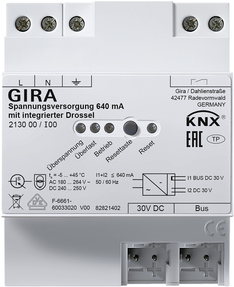
\includegraphics[width=0.3\textwidth]{figures/fuente_alimentacion.png}   
\caption{Fuente de alimentación}
\label{fig:fuente_alimentacion}
\end{figure}

  
\chapter{Estado del Arte}

Con muy pocos años de rodaje, la domótica se ha convertido en uno de los sectores con mayor relevancia y perspectiva de incremento y potenciación futura, gracias a los avances tecnológicos recogidos en numerosos artículos y publicaciones, como el caso de “Domótica: Edificios Inteligentes” \cite{EI:2004}. Estos avances que van de la mano de otros sectores como por ejemplo, el social con su continua lucha hacia la inclusión total de la población o el diseño de interiores y su afán por convertir nuestros hogares en una prolongación más de nuestro cuerpo, para hacernos sentir lo más cómodos y confortables posible. Pero es, sin duda, la apuesta de la sociedad por la inclusión de esta tecnología en el sector de la construcción lo que provoca su gran avance, mejorando e incluso desarrollando nuevas funcionalidades, lenguajes de programación y protocolos de comunicación.\\\\
Esta evolución ha ido permitiendo de manera progresiva que, poco a poco los sistemas domóticos integren una mayor cantidad de mecanismos, ampliando así el catálogo de funcionalidades que pueden ofrecer, a la par que estos son diseñados para actuar de manera más independiente y autónoma. En un principio, los sistemas domóticos eran centralizados, es decir, todos los mecanismos y sus parámetros eran controlados desde una central; en cambio, a día de hoy, los elementos son inteligentes y pueden portar su propia programación, y actuar en consonancia a ella, convirtiéndose en sistemas descentralizados. Esta cualidad, obtenida con el paso del tiempo y la integración de los avances tecnológicos, ha permitido la mejora de 4 áreas fundamentales en el control de una vivienda: la seguridad, la gestión energética, el confort y las comunicaciones  \cite{Andes:2011}, como se demostró en la Universidad Católica del Ecuador \cite{Ecuador:2017}, donde gracias a la mejora de los protocolos de comunicación, en especial, la implementación del X10, se pudo domotizar una escuela al completo, mejorando así la calidad de la enseñanza y la satisfacción de sus alumnos y profesores.\\\\
En el caso del ámbito de la seguridad doméstica, la domótica explota de manera mucho más eficiente que los sistemas tradicionales, en al menos 3 de los campos más demandados, integrándolos con el resto de dispositivos. Uno de estos campos será el enfocado hacia las alarmas técnicas, que mediante sistemas sensoriales, podrán avisar al usuario de que existe un elemento en la casa que se encuentra averiado o realizando un mal funcionamiento, como pueda ser una tubería de agua rota o un horno demasiado caliente que quema la comida. Si el problema cuenta con una mayor gravedad o se requiere controlar espacios de manera más certera, incluso se podrán conectar estas alarmas con los servicios de emergencia o reparación profesionales, como pueden ser los bomberos. \\\\
Haciendo uso de esa misma capacidad de conectar con sistemas externos, encontramos los otros 2 campos: la seguridad de los bienes, que mediante detectores de presencia y diferentes actuadores, como alarmas sonoras o cegadoras, tratara de evitar la entrada o sustracción de bienes de la vivienda, enviando un aviso al cuerpo de policía; y la teleasistencia, muy útil especialmente para personas mayores o enfermas, que podrán conectar con los servicios sanitarios que requieran con la simple pulsación de un botón.\\\\
En cuanto a la gestión energética, la domótica también se ha hecho un hueco en este sector gracias a la integración de elementos como temporizadores, termostatos, relojes temporizadores con otros más habituales, como los contadores de consumo, que conectados a través de actuadores, crean un sistema eficiente de ahorro de energía.\\\\

Desde el comienzo de su aplicación en los años 80, principalmente en EE.UU. y Japón, y su popularización en los 90 en países de Europa como Francia, Alemania u otros países nórdicos, la domótica ha ido de la mano del mercado de la construcción. Este sector, ya desde 2004, impulsaba el crecimiento del uso de la domótica al ser instalado en el 7\% \cite{Ikei:2004} de las nuevas promociones, propiciando la aparición de comités de expertos que comienzan a regular y afianzar el termino domótica, creando en Europa en 2006 la Especificación de AENOR EA2006 \cite{direct:2004}, pionera de este sector, que determinaría los requisitos mínimos que debía dispensar una vivienda para poder ser considerada domótica. Una vez fijados la base del concepto, instituciones  como el Ministerio de Industria y Turismo pronto comenzaron a realizar otro conjunto de guías y manuales, como por ejemplo, la Guía Técnica de Aplicación ITC-BT-51 \cite{BOE:2002} creada en 2007, que sentaba catedra acerca de “los requisitos específicos de la instalación de los sistemas de automatización, gestión técnica de la energía y seguridad para viviendas y edificios, también conocidos como sistemas domóticos”.\\\\ 
El estallido de la burbuja inmobiliaria acompañado a la crisis financiera global de finales de la primera década del siglo provoco una caída del 62\% en la construcción de nuevas viviendas, truncando la tendencia a la alza que tenía el mercado domótico, llegando a traducir su incidencia en un descenso del 60\% de la instalación en vivienda nueva \cite{AED:2011}, lejos de la previsiones vaticinadas por numerosos medios \cite{mundo:2010} \cite{Info:2008}, que predecía un 25\% de viviendas de nueva obra con instalación domótica integrada en el año 2010.\\\\
 La domótica, actualmente, se encuentra en continuo desarrollo y enfrentándose a diversos conflictos o problemas como su alto coste de instalación, la falta de personal cualificado, la normalización de los diversos softwares que existen en los diferentes mercados del mundo, la dependencia del sistema eléctrico o los problemas del mundo de la informática, como pueden ser los hackers \cite{cerda:2018}, dando sensación de inseguridad dentro de la tu propia casa. Por lo tanto, es una ciencia con un potencial muy grande pero debe superar los problemas básicos con que se encuentra cualquier tecnología durante su fase de desarrollo, para poder crecer y convertirse en un referente en cuanto a los servicios que ofrece y lo óptimo de sus resultados.\\\\
A día de hoy, ya se ha implementado en 44 millones de hogares en Europa y Norte América \cite{HT:2014}, brindando así la certeza del potencial con el que cuenta esta tecnología y el crecimiento exponencial en el que se encuentra: en 2015, en Europa existían únicamente 5.3 millones de viviendas frente a los 18 millones de 2020. Esta cifra lejos de congelarse, continua en crecimiento con la meta de alcanzar un 20\% de casas domotizadas del total en Europa para el año 2025 \cite{Berg:2020}. En cuanto a su desarrollo en España, se espera que el auge de la domótica logre alcanzar un 300\% para el año 2024, realizándose en casi un 60\% de instalaciones de nueva construcción \cite{Portal:2020} y encontrándose ya en el 40\% de los hogares en forma de dispositivo inteligente



\chapter{How to write in Latex}

\section{Estilo}

Al ser un documento científico-técnico, debe ser expuesto en tercera persona del singular. También se admite usar la primera persona cuando son apreciaciones personales del autor.

\section{Citas}

%las referencias a artículos se ponen con \cite, 
%las referencias a imágenes \ref, 
%y las referencias a ecuaciones \eqref

Esto es un ejemplo de cita de un artículo \cite{Brunete:2013}.


\section{Listas}

%itemize es una lista. Cada término lleva delante un \item
Ejemplo de lista de puntos:
\begin{itemize}
\item Ejemplo1.
\item Ejemplo2.
\end{itemize} 

Y lista numerada:
\begin{enumerate}
\item Elemento 1
\item Elemento 2
\end{enumerate}

\section{Tablas}

Ejemplo de tabla. Como se aprecia en la tabla \ref{tab:table_example}...
\begin{table}[tb]
\caption{Ejemplo de tabla}
\label{tab:table_example}
\begin{center}
\begin{tabular}{|c||c|c|}
\hline
One & Two & Three\\
\hline
\hline
F1A & F1B & F1C\\
F2A & F2B & F2C\\
\hline
\end{tabular}
\end{center}
\end{table}

\section{Referencia a una sección}
\label{sec:refsec}

Ejemplo de referencia a la sección \ref{sec:refsec}

\section{Texto}

Texto en \textbf{negrita} y \textit{cursiva}.

\section{Figuras}

Ejemplo de referencia a figura (figura \ref{fig:logo_upm}). Es importante que todas las figuras que aparezcan estén referenciadas, así como las tablas. En general las figuras se colocarán al principio o al final de cada página ([tb] en latex), a no ser que por alguna necesidad se deban colocar en una posición exacta ([h]).

%caption es el pie de foto, y label es el nombre que se da a la imagen para referenciarla después. label no puede llevar acentos y no se muestra de cara al documento final (es sólo interno).
\begin{figure}[tb]
\centering

\includegraphics[width=0.45\textwidth]{figures/Logo_UPM.jpg}   
\caption{Logotipo de la UPM}
\label{fig:logo_upm}
\end{figure}

\textbf{Muy importante!: Todas las figuras no originales que aparezcan en la memoria deben ir referenciadas.}


\section{Código software}

Existen muchas formas de escribir código en el TFG. Aquí se muestra una de ellas. En general es interesante numerar las líneas para que sean referenciables y destacar palabras clave del lenguaje correspondiente. Ver código \ref{code:prog1}.

% Esto para configurar como se va a visualizar el código
\lstset{numbers=left,numberstyle=\tiny, language=C, breaklines=true, basicstyle=\footnotesize, xleftmargin=25pt, framesep=8pt, numbersep=15pt}


\begin{lstlisting}[frame=leftline, caption={Hola Mundo}, label=code:prog1]
#include <iostream> 

using namespace std;

int main(int argc, char *argv[]) {
  cout << ``Hola mundo'' << endl;
  return 0;
}
\end{lstlisting}


En general no se debe incluir mucho código en la memoria. El código debe ir en el Anexo. 

\section{Pie de página}

Esto es un pie de página \footnote{Pie de página}. Y para usar direcciones web y no tener problemas con caracteres especiales (como el ``\_''), se usa el comando url \footnote{\url{https://es.wikipedia.org/wiki/Estado_del_arte}}





\include{chapters/diseño}

\chapter{Desarrollo del proyecto}

En este capítulo se describe el desarrollo del proyecto

\section{Direcciones de grupo y objetos de comunicación}
\label{sec:dir_grup}

Al utilizar el estándar de programación de KNX, será necesaria la creación de las direcciones de grupo del sistema, cuya función principal será la de actuar como nexo de comunicación entre los diferentes objetos de comunicación con los que cuentan los módulos. Todos los objetos de comunicación cuentan con seis \textit{flags} distintos seleccionables en función de la ocupación que vayan a desarrollar, a saber:
\begin{itemize}
\item \textit {C-flag}: es el \textit{flag} de comunicación (\textit {Communication}), y tal y como indica su nombre, su función será la de abrir y permitir el canal de comunicación hacia ese objeto de comunicación del módulo. Por lo general, es un \textit{flag} que se encuentra activo en prácticamente todos los objetos, y solo será deshabilitado en situaciones muy concretas en las que su no actuación sea crítica.
\item \textit {R-flag}: es el \textit{flag} de lectura (\textit {Read}), y permite al objeto de comunicación ser consultado por su valor, como si de una variable de programación se tratase. Este \textit{flag} se encuentra activo principalmente en aquellos objetos que devuelven el estado de un parámetro del sistema, como por ejemplo, el estado en que se encuentra una de las salidas de un actuador ON/OFF. Cuando otro objeto trate de comunicarse con él, contestará con el valor actual en el que se encuentra, 0 ó 1, siguiendo con el ejemplo anterior, pero pudiendo ser un valor de la posición en porcentaje de apertura de una ventana o el valor de la temperatura de consigna establecida en ese momento en el módulo. Son usados para representar el estado de las variables en una interfaz gráfica para poder ser consultados por el usuario.
\item \textit {T-flag}: se trata del \textit{flag} de transmisión (\textit {Transmit}), el cual cuanta con bastante similitud con el \textit {R-flag}, con la salvedad de que este objeto no espera a ser consultado para enviar su valor, sino que lo enviará siempre que se produzca un cambio de valor en él. Un ejemplo de este comportamiento, lo podemos encontrar en los objetos de comunicación que reciben el estado de un sensor, enviando la actualización de su valor en cuanto que esta se produce.
\item \textit {W-flag}: es el \textit{flag} de escritura (\textit {Write}), y será aquel que recibe el valor de la variable desde los actuadores físicos, los \textit{R-flag} o los \textit{T-flag} y les permite sobrescribir su valor. Esto es muy útil a la hora de que exista varios puntos de control de un mismo elemento y todos conozcan y se encuentren con el mismo valor, actuando a su vez sobre los elementos hardware de la instalación. Por ejemplo, al ejecutar una pulsación sobre un interruptor, este \textit{flag} permitirá que el objeto de comunicación modifique su valor de 0 a 1, o viceversa, enviando la orden al actuador para que abra o cierre el relé correspondiente.
\item \textit {U-flag}: es el \textit {flag} de actualización (\textit {Update}), cuya misión es simplemente la de buscar de manera continua algún tipo de modificación en los estados, para así modificar su valor de manera automática. Estos \textit{flags} no suelen ser muy utilizados en objetos de comunicación que cuenten con \textit {R-flag} o \textit {T-flag}, ya que se producen bastantes errores al leerse a sí mismos, provocando bucles de realimentación de estado durante tiempos indefinidos, ocupando la línea de comunicación del bus, dando lugar a un colapso en ella. Se suelen activar con \textit {W-flag}, permitiendo así su autoreescritura en cuanto se produce algún cambio en sus asociaciones.
\item \textit {I-flag}: se trata del \textit {flag} que permite al objeto de comunicación adoptar un valor al inicio (\textit {Initialization}) de su funcionamiento o tras una caída en la tensión del bus o cualquier otro problema relacionado con la perdida de comunicación del módulo con el resto del sistema.
\end{itemize}
Todos estos \textit {flags} pueden ser activados en todos y cada uno de los objetos de comunicación, aunque su activación no implica que realmente vaya a cumplir con esa funcionalidad, ya que también se requiere que el hardware de su módulo pueda físicamente ejecutarlo. Un ejemplo del comportamiento más usual en las comunicaciones con protocolo KNX lo vemos representado en la Imagen \ref{fig:diag_flags},  donde podemos ver que el objeto de comunicación textit {ON/OFF Luz Cocina} se inicializa con el valor 0 preprogramado gracias a su \textit {I-flag} y se envía la orden al actuador por tener el textit {W-flag} activo. Una vez que el actuador, en este ejemplo, abra el relé, el objeto de comunicación textit {STD ON/OFF Luz Cocina} recoge el estado en que se encuentra esa salida debido a que este objeto tiene en funcionamiento su \textit {R-flag}. De este objeto de comunicación se harán lecturas de ese valor desde otros objetos de comunicación que se encuentren ligados a él en la misma dirección de grupo, como pueden ser los LEDs de dos pulsadores y un icono de la interfaz gráfica que representan este estado, que gracias a su \textit {W-flag}, actualizarán su valor a 0.\\\\
Si ahora se pulsase el pulsador P1, este escribiría un 1 en el objeto de comunicación textit {ON/OFF Luz Cocina}, lo que provocaría que el actuador cerrase el relé, permitiendo la circulación de la corriente y por tanto, el encendido de la bombilla. En ese momento, el objeto de comunicación textit {STD ON/OFF Luz Cocina} detecta el cambio de estado de la salida del actuador, y actualiza su valor a 1, volviendo a permitir que, no solo P1, si no también P2 y la pantalla, actualicen su estado y enciendan sus LEDs informativos y el icono cambiase a su representación de luz encendida. De esta manera el usuario es capaz de conocer el estado de un elemento de manera remota. Si ahora se diese el caso de que se pulsase el pulsador P2 o se actuase desde la pantalla, al conocer el estado en que se encuentra actualmente la luz, enviarán el valor contrario mediante una acción de textit {switch}, en este caso 0, volviendo a actuar sobre el actuador pero a la vez informando al resto de módulos del estado de ese elemento, tal y como sucedió al actuar sobre P1.
 \begin{center}
\begin{figure}[H]
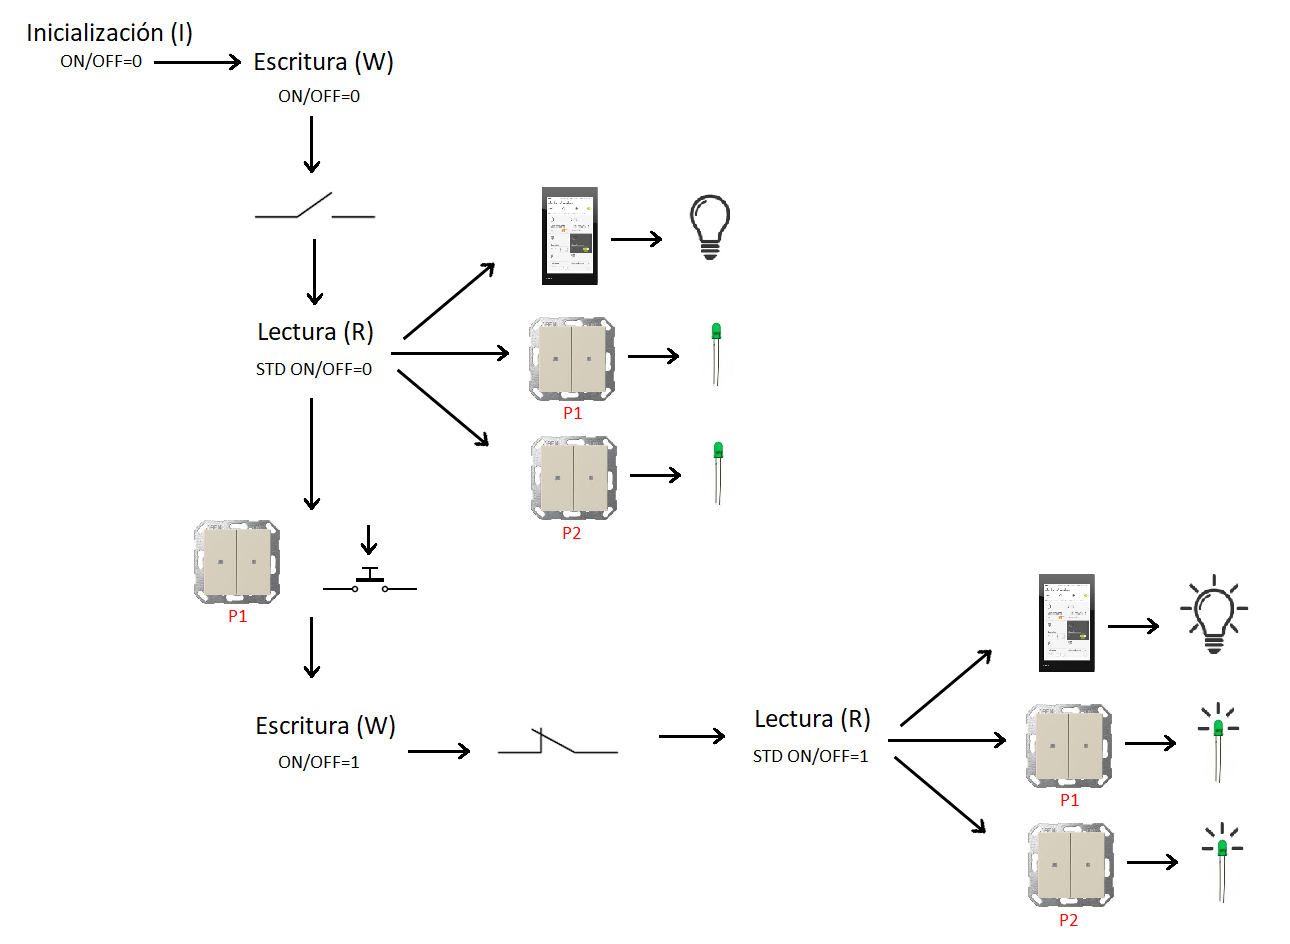
\includegraphics[width=1.15\textwidth]{figures/diag_flags.png}   
\caption{Diagrama uso de flags}
\label{fig:diag_flags}
\end{figure}
\end{center}
Como se comentaba al comienzo de este capítulo, los objetos de comunicación de los mecanismos se comunican entre sí al linkarse a la misma dirección de grupo, como es el caso de los LEDs de los pulsadores y el icono de la pantalla, que están linkados a la dirección de grupo denominada textit {ON/OFF Luz Cocina}. Estas direcciones han de ser creadas por el programador en función de las tareas y acciones que desee realizar en la instalación. Para una mayor organización, el software ETS5 ofrece tres niveles de dirección de grupo: el principal, que da información acerca de que sección se controla, uno intermedio, que anuncia que funcionalidad se ejecuta, y finalmente las propias direcciones de grupo, que llevarán el nombre concreto del efector y la función que utiliza. Siguiendo con el ejemplo de la Imagen \ref{fig:diag_flags},  el nivel superior llevaría el nombre de textit {Iluminación} con el número 1, el intermedio textit {ON/OFF} con la identificación 1/1, y finalmente, y tal como se comentó, la dirección de grupo será nombrada como textit {ON/OFF Luz Cocina}, con tipificación 1/1/1. De esta manera, se establece una jerarquía organizativa que permite a los instaladores o incluso programadores futuros que modifiquen el proyecto, localizar las direcciones de grupo de manera más intuitiva y sencilla.
\newpage
En este proyecto se ha creado la siguiente jerarquía de organización para contener todos los objetos de comunicación que van a ser utilizados durante el funcionamiento de la instalación:

\begin{multicols}{2} 
\begin{flushleft} 
\begin{itemize}
\item{0 General}
\begin{itemize}
\item{0/1 Escenas}
\item {0/2 Parámetros del sistema}
\end{itemize} 
\end{itemize} 
\vspace{1.5cm}
\end{flushleft} 

\begin{flushright}  
\begin{itemize}
\item{1 Iluminación}
\begin{itemize}
\item{1/1 ON/OFF}
\item{1/2 STD ON/OFF}
\item{1/3 DIMMING}
\item{1/4 VALOR DIMMING}
\item{1/5 STD VALOR DIMMING}
\end{itemize} 
\end{itemize} 
\end{flushright} 
\end{multicols} 

\begin{multicols}{2} 
\begin{flushleft} 
\begin{itemize}
\item{2 Persianas, Proyector y Puerta}
\begin{itemize}
\item{2/1 UP/DOWN}
\item{2/2 STEP/STOP}
\item{2/3 VALOR}
\item{2/4 STD VALOR}
\item{2/5 TIMBRE}
\item{2/6 PUERTA}
\end{itemize} 
\end{itemize} 
\vspace{0.5cm}
\end{flushleft} 

\begin{flushright} 
\begin{itemize}
\item{3 Climatizacion}
\begin{itemize}
\item{3/1 ON/OFF}
\item{3/2 STD ON/OFF}
\item{3/3 MODO CLIMA}
\item{3/4 STD MODO CLIMA}
\item{3/5 TEMP CONSIGNA}
\item{3/6 STD TEMP CONSIGNA}
\item{3/7 TEMP REAL}
\end{itemize} 
\end{itemize} 
\end{flushright} 
\end{multicols} 

\begin{multicols}{2} 
\begin{flushleft} 
\begin{itemize}
\item{4 Variables climatizacion}
\begin{itemize}
\item{4/1 POS REJILLA}
\item{4/2 STD POS REJILLA}
\item{4/3 VEL FAN}
\item{4/4 STD VEL FAN}
\item{4/5 MODO FAN}
\item{4/6 STD MODO FAN}
\item{4/7 STD VENTANA}
\end{itemize} 
\end{itemize} 
\end{flushleft}

\begin{flushright} 
\begin{itemize}
\item{5 Consumo}
\begin{itemize}
\item{5/1 SOLICITUD}
\item{5/2 CAUDAL AGUA (l/h)}
\item{5/3 CAUDAL GAS (m3/s)}
\item{5/4 POTENCIA (kW)}
\item{5/5 ENERGIA (kW•h)}
\item{5/7 FECHAS}
\end{itemize} 
\end{itemize} 
\end{flushright} 
\end{multicols} 

\begin{multicols}{2} 
\begin{flushleft} 
\begin{itemize}
\item{6 CO\textsubscript{2} y Recuperador}
\begin{itemize}
\item{6/1 LIMITES CO2}
\item{6/2 ON/OFF FAN CO2}
\item{6/3 STD ON/OFF FAN CO2}
\item{6/4 VEL FAN CO2}
\item{6/5 STD VEL FAN CO2}
\item{6/6 MEDIDA CO2}
\end{itemize} 
\end{itemize} 
\end{flushleft}

\begin{flushright} 
\begin{itemize}
\item{7 Detectores y efectores}
\begin{itemize}
\item{7/1 ON/OFF ELECT. VALV.}
\item{7/2 STD ELECT. VALVULAS}
\item{7/3 SIRENA HUMO}
\item{7/4 STD SIRENA HUMO}
\item{7/5 STD DETECTORES}
\end{itemize} 
\end{itemize} 
\end{flushright} 
\end{multicols} 

\begin{flushleft} 
\begin{itemize}
\item{8 Centralizados}
\begin{itemize}
\item{8/1 ILUMINACION}
\item{8/2 CLIMA}
\item{8/3 PERSIANAS}
\end{itemize} 
\end{itemize} 
\end{flushleft}

A continuación, se realiza una breve explicación de que significa cada una de estas direcciones de grupo de nivel medio para facilitar la comprensión de esta clasificación:
\begin{itemize}
\item Estados: por norma general, todas las direcciones de grupo de acciones llevan asociada una dirección de estado, nombradas como STD y que contienen el mismo tipo de variables, para realizar la lectura del estado del efector que ha sido modificado. Serán del mismo tamaño que la acción a la cual se encuentran referenciadas.
\item Dimming: este tipo de datos será el encargado de enviar los telegramas que indican a los mecanismos si deben “subir” o “bajar”, como es el caso de la posición de una persiana o el de regular la intensidad de una bombilla. Cuentan con un tamaño de 4 bits.
\item Up/Down: envía la orden de subir o bajar mediante el envio de un 0 ó un 1, por lo que su longitud de paquete será de 1 bit.
\item Step/Stop: permite enviar un telegrama que indique al mecanismo que debe para en su regulación o dar un “paso” preajustado (normalmente del 12.5\% del total), tanto de “subida” como de “bajada”. Su tamaño es de 1 bit.
\item Valor dimming o posición: esta dirección permitirá al usuario enviar un valor porcentual concreto al elemento regulable, para establecer su nivel de “subida” y “bajada” en una posición concreta. Por ejemplo, permite enviar un “50\%” a una lámpara, para que se regule a la mitad de su máxima intensidad lumínica. En esta ocasión, el tamaño de esta variable será de 1 byte, ya que se requerirá mayor espacio para enviar el valor del porcentaje con una precisión de 1/256.
\item Temperaturas: esta clase de direcciones permitirá transmitir valores de tipo temperatura, que contarán con 2 bytes de memoria para permitir los valores decimales, ofreciendo así la posibilidad de regular con mayor precisión las temperaturas deseadas en la vivienda.
Valores de lectura: estos parámetros son utilizados para hacer lecturas de los sensores implementados en el sistema. Debido a la gran variedad de estos, no poseen un tamaño fijo y su valor fluctuará desde 1 bit, como en el caso de un sensor de detección de ventana abierta/cerrada, hasta un máximo de 4 bytes, como en la lectura del caudal de gas.
\item Centralizados: este tipo de dirección permite agrupar diversos objetos de comunicación para que los mecanismos se comporten todos de la misma manera en el mismo instante. Su funcionalidad es totalmente abierta, y por tanto su tamaño dependerá de la acción que se ejecute. Los centralizados son utilizados en este proyecto para realizar un apagado general del sistema de iluminación (1bit) o para hacer un control sobre la posición de todas las persianas (1 byte), permitiendo así situarlas todas en la misma posición proporcional.
\item Escenas: estas direcciones tienen una lógica similar a la de los centralizados, con la salvedad de que estos permiten enviar diferentes órdenes a los mecanismos de manera simultánea. Una escena que se ha programado en este proyecto, recibe el nombre de “Salir de casa”, y en ella se ejecuta el apagado de todas las luces de la vivienda, se bajan todas las persianas y se desactiva el recuperador de CO\textsubscript{2}.
\end{itemize} 

\section{Programación de los mecanismos}

Una vez explicada la base de trabajo de la programación, en este capítulo se pasará a comentar el linkado que se ha establecido entre los diferentes objetos de comunicación de los módulos instalados en la vivienda y las direcciones de grupo creadas y comentadas con anterioridad. También se detallarán los bloques lógicos creados para satisfacer los requisitos del cliente en aquellas ocasiones que los objetos de comunicación predefinidos de los módulos no llegan al alcance requerido de precisión o funcionalidad, y por tanto, es necesaria la implementación de una programación complementaria. Los bloques lógicos son una variedad de funciones del tipo \textit {drag and drop} que ofrece el servidor X1 y permite crear entramados complejos de pautas de funcionamiento mediante la asociación de \textit {“cajas lógicas”} que manipula, transforma o asocia direcciones de grupo. En esta sección se explicará en detalle también la lógica aplicada durante el diseño de estos bloques lógicos.

\subsection{Iluminación} Esta sección entrelazará los pulsadores domóticos con los actuadores, tanto binarios como reguladores, a través del bus KNX para poder actuar sobre el sistema de iluminación de la vivienda a través de la dirección de grupo ON/OFF. A las teclas de los pulsadores que se encargarán del apagado, encendido y regulación de luminarias, se les ha otorgado la funcionalidad de conmutación con aplicación de tipo \textit {“switch”}, permitiendo así el envío del valor binario adecuado (contrario al existente en el momento) al accionar el pulsador. Por otro lado, se han programado ambas clases de actuadores para que en caso de caída de tensión en el bus, recuperen de su \textit {stack} de memoria el último valor en el que se encontraban las luces previamente. \\\\
El funcionamiento básico de esta sección hace de su programación una tarea sencilla y sin ningún tipo de complejidad, pero por solicitud del cliente ha sido necesario implementar un complejo bloque lógico para lograr controlar las lámparas dimmeables desde el único punto de los pulsadores KNX. El funcionamiento esperado sigue las siguientes pautas: con una pulsación larga, la lámpara comienza a aumentar su intensidad lumínica si la acción durante la última pulsación larga había sido reducir el valor lumínico. Por el contrario, si la última acción había sido aumentar de tensión, al realizar una pulsación larga, debe comenzar a descender su intensidad. \\
Por otro lado, y en cuanto a la pulsación corta, si se da mientras no se esté ejecutando ninguna regulación: si la luz se encuentra encendida, pasará a estar apagada, mientras que si se encontraba apagada, regulará de manera automática y progresiva la intensidad lumínica hasta el valor guardado en el \textit {stack} de memoria en el momento de parar la regulación.
\newpage
 El diagrama de bloques diseñados en el módulo X1 es el siguiente:
 \begin{center}
\begin{figure}[H]
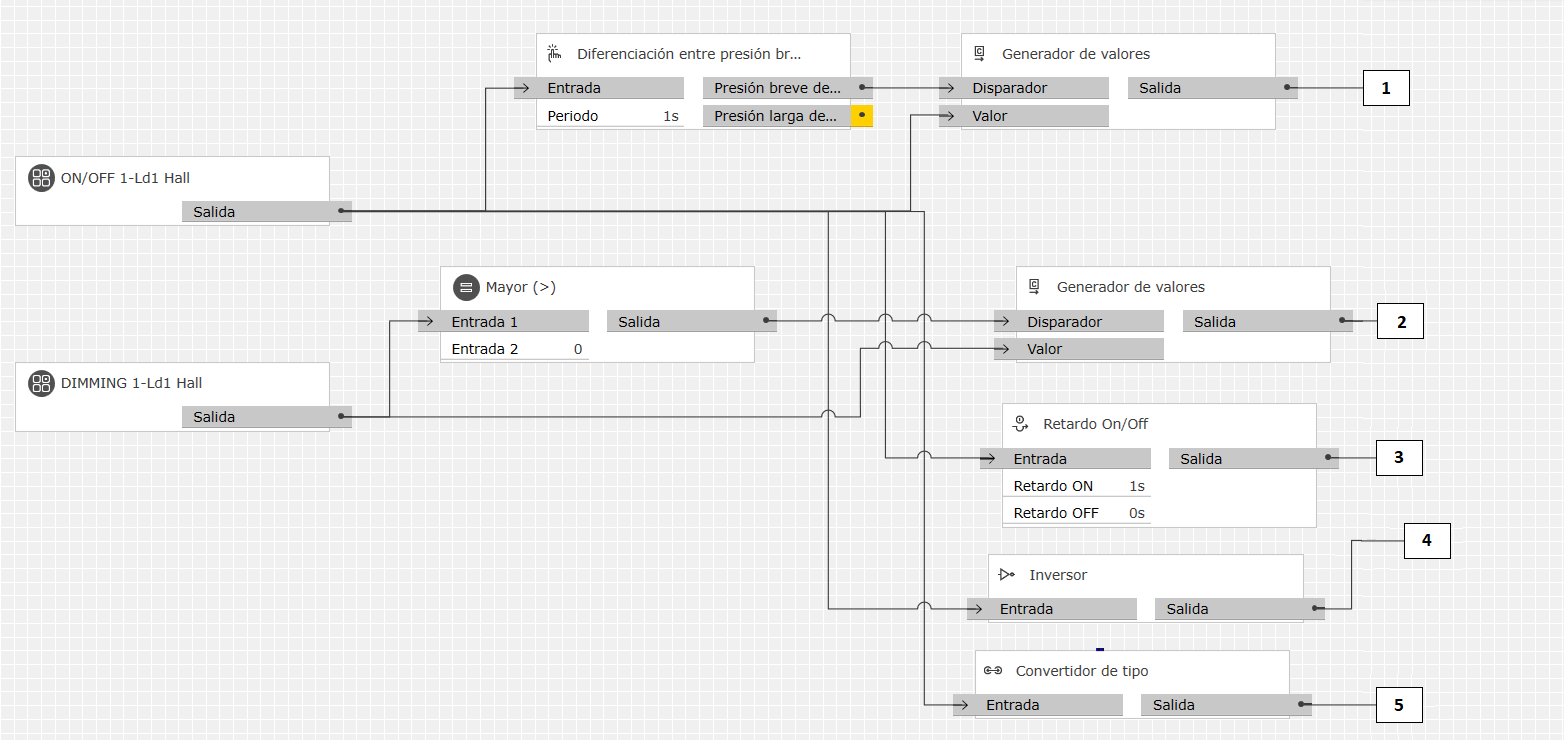
\includegraphics[width=1.05\textwidth]{figures/log_dimm_izq.png}   
\caption{Módulo lógico DIMMER (1ª Parte)}
\label{fig:log_dimm_izq}
\end{figure}
\end{center}
 \begin{center}
\begin{figure}[H]
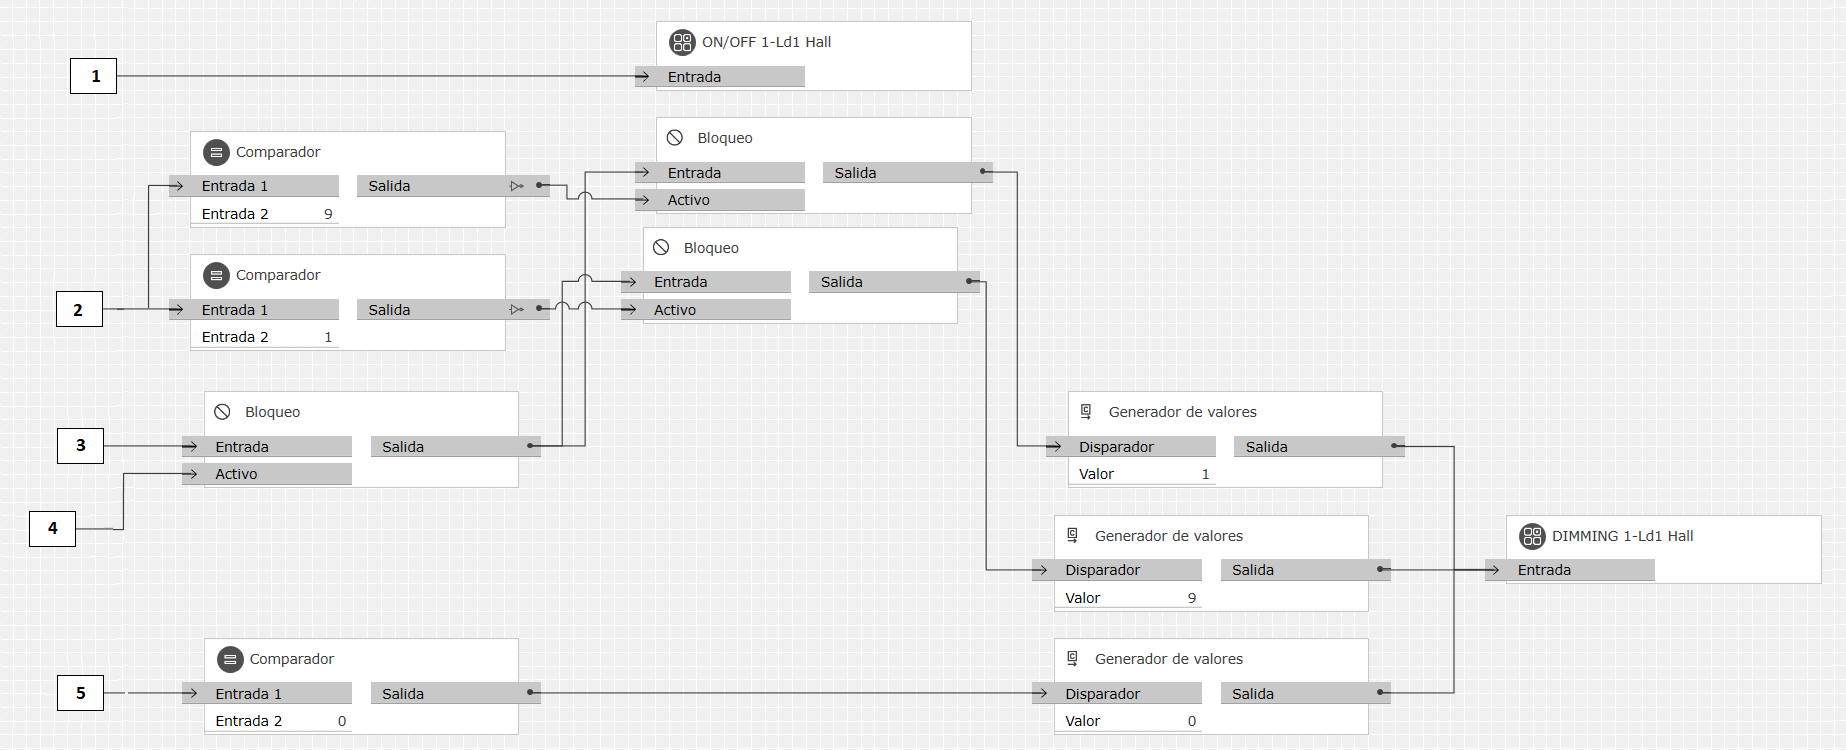
\includegraphics[width=1.05\textwidth]{figures/log_dimm_der.png}   
\caption{Módulo lógico DIMMER (2ª Parte)}
\label{fig:log_dimm_der}
\end{figure}
\end{center}
En él podemos encontrar dos entradas de datos: la señal de ON/OFF de la luminaria y la orden de DIMMER, que atacarán a sus homologos de las salidas, una vez realizadas todas las secuencias del bloque lógico, que a continuación será descrito: 
\newpage
Por un lado, la señal de ON/OFF se envía a un bloque lógico capaz de diferir entre una pulsación larga de una corta, preestableciendo el valor que las diferencia durante su programación, en este caso, de un segundo. Este bloque ha sido programado para que únicamente se obtenga una señal de salida de valor “1” cuando la pulsación que es detectada es breve, y es enviada al disparador de un bloque Generador de valores. Este bloque tiene la función de que en el momento que recibe un “1” por su puerto “Disparador”, envía el valor recibido por su puerto “Valor”, que en este caso, es la propia señal de ON/OFF de la entrada. Este valor será recibido por un bloque de salida, que es el encargado de modificar el valor de la propia dirección de grupo ON/OFF de la lámpara.
\begin{center}
\begin{figure}[H]
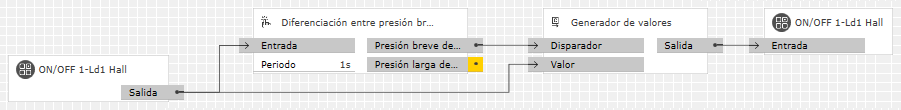
\includegraphics[width=1.15\textwidth]{figures/log_dimm_b1.png}   
\caption{Módulo lógico DIMMER: bloque 1}
\label{fig:log_dimm_b1}
\end{figure}
\end{center}
Con estos módulos lo que se logra simular es el encendido y apagado de la bombilla regulada desde el actuador de regulación al hacer una pulsación corta sobre el pulsador domótico.\\\\
A continuación, encontramos la segunda entrada, en este caso apuntando hacia la dirección de grupo DIMMING, la cual, en primera instancia, entrará a un bloque lógico Comparador. Este bloque se ha configurado para que su salida sea un “1” cuando el valor de entrada sea mayor que 0. Tanto para el valor de subida como de bajada, el valor de este telegrama será mayor de 0, respectivamente y en valores binarios, 101 y 001. En estos dos  casos, la salida del comparador será un “1”, que irá direccionado al puerto “Disparador” de otro bloque Generador de valores, cuyo valor de salida al activarse será el propio valor de la entrada de DIMMER. \\ Este valor será enviado a dos bloques Comparadores, uno programado para identificar unos y otro para nueves, cuyas salidas irán invertidas y direccionadas a la entrada de activación de un módulo de Bloqueo cada una. Estos módulos tienen un funcionamiento bastante sencillo e intuitivo: actúan como de buffer de datos, que entran por su puerto “Entrada”, siempre que reciban un “0” por su puerto “Activo”, puesto que si por el contrario reciben un “1”, bloquearan el envío de ese valor. 
 \begin{center}
\begin{figure}[H]
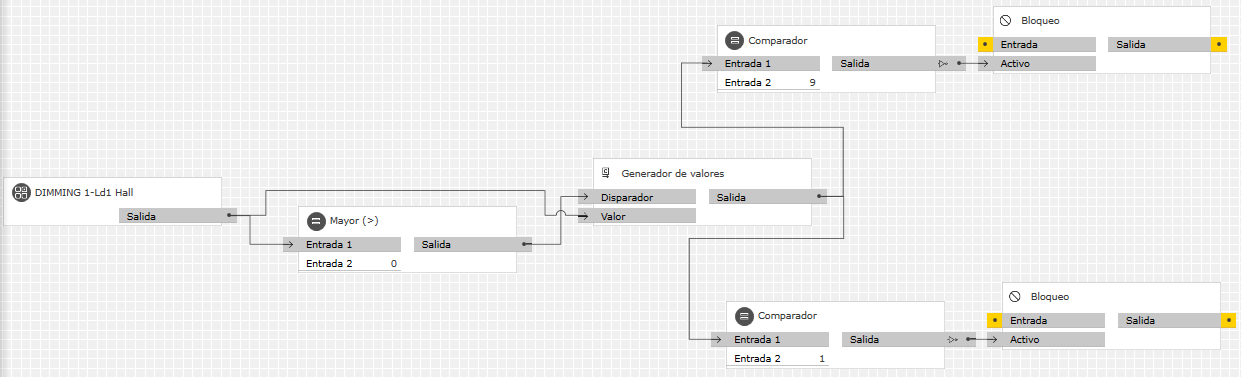
\includegraphics[width=1.15\textwidth]{figures/log_dimm_b2.png}   
\caption{Módulo lógico DIMMER: bloque 2}
\label{fig:log_dimm_b2}
\end{figure}
\end{center}
Por otro lado, los valores que se envían una vez que estos módulos de Bloqueo son desactivados provienen del tratamiento de la entrada ON/OFF. Esta señal en primer lugar pasará por un bloque lógico de Retardo ON/OFF, el cual permite seleccionar el tiempo de retardo del envío de las señales de ON/OFF, que en esta ocasión únicamente se ha establecido en 1 segundo para el ON, manteniendo el envío instantáneo para el OFF. A continuación, estos valores irán a la entrada de otro módulo de Bloqueo, cuya señal de activación es el valor invertido de la propia señal ON/OFF al pasar a través de un bloque Inversor, logrando así únicamente transmitir el “1” generado al activar la señal de ON/OFF, siendo este “1” las señales de entrada y valor a transmitir de los módulos de Bloqueo activados por los bloques Comparadores de unos y nueves mencionados anteriormente, cuya función era la de activarlos y desactivarlos. Una vez que estos bloques se encuentran desactivados y permiten el paso del valor, este se dirige a la entrada disparador de un Generador de señales, uno por cada módulo de Bloqueo, que transmitirán un uno o un nueve a la salida de DIMMING, según cuál de ellos sea activado.
 \begin{center}
\begin{figure}[H]
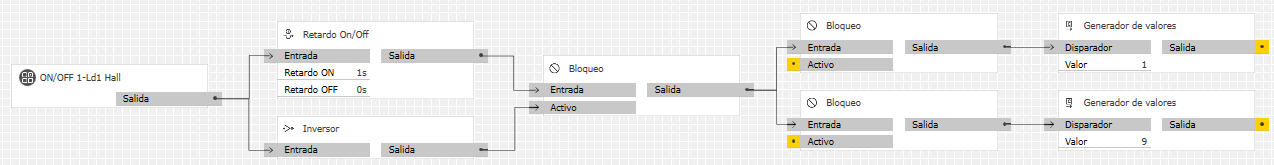
\includegraphics[width=1.15\textwidth]{figures/log_dimm_b3.png}   
\caption{Módulo lógico DIMMER: bloque 3}
\label{fig:log_dimm_b3}
\end{figure}
\end{center}
En último lugar, la señal de ON/OFF volverá a ser utilizada, siendo en primer lugar por un bloque Convertidor de tipo, configurado para obtener a su salida un valor binario de esta entrada. Una vez convertido, este valor pasará a un bloque Comparador programado para  contrastar si el valor recibido es un “0”, y enviar un “1” al puerto disparador de un bloque Generador de valores, que enviará un cero a la salida de DIMMING una vez se dispare. 
 \begin{center}
\begin{figure}[H]
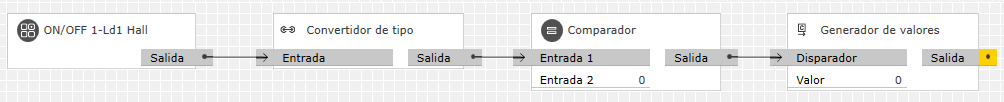
\includegraphics[width=1.15\textwidth]{figures/log_dimm_b4.png}   
\caption{Módulo lógico DIMMER: bloque 4}
\label{fig:log_dimm_b4}
\end{figure}
\end{center}
Con la unión de los paquetes lógicos 2, 3 y 4 lo que se logra es hacer un envío cíclico y ordenado de los valores de dimming de subida y bajada de tensión, que serán alternados a través del uso de los paquetes 2 y 3, que enviarán alternativamente los valores “1” y “9” correspondientes con la orden de bajada y subida respectivamente, mientras que el valor “0” será enviado siempre a la salida de DIMMING cuando se produzca en la entrada ON/OFF, simplemente para que esa dirección de grupo actualice su estado de cara al próximo proceso de regulación de esa lámpara o bien para actualizar su estado en las interfaces gráficas que utiliza el cliente.
 \begin{center}
\begin{figure}[H]
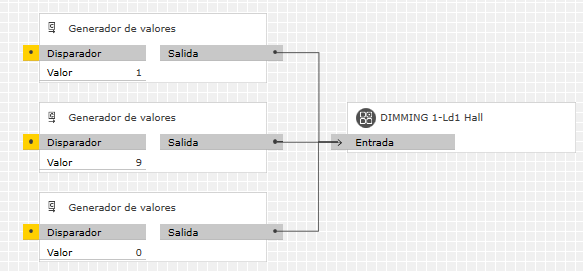
\includegraphics[width=0.95\textwidth]{figures/log_dimm_b5.png}   
\caption{Módulo lógico DIMMER: bloque 5}
\label{fig:log_dimm_b5}
\end{figure}
\end{center}
En la siguiente imagen se muestra los linkados dados en las direcciones de grupo de una luminaria de tipo regulable:
 \begin{center}
\begin{figure}[H]
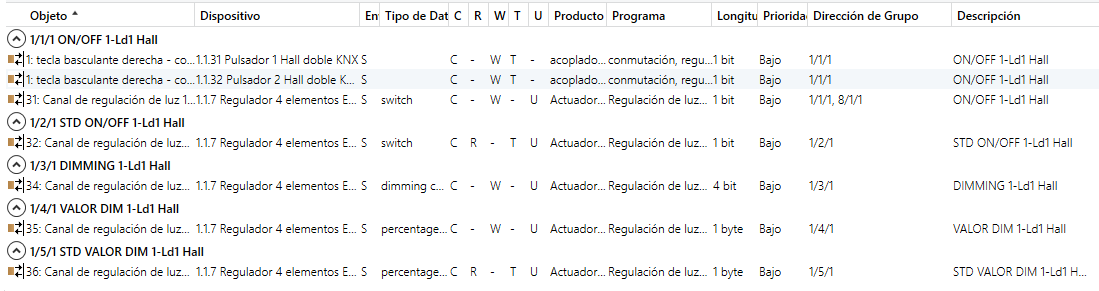
\includegraphics[width=1.15\textwidth]{figures/prog_dim.png}   
\caption{Programación genérica de la sección de Iluminación}
\label{fig:prog_dim}
\end{figure}
\end{center}

\subsection{Persianas/ventanas}Como ya se comentó en la sección \ref{sec:dir_grup}, las persianas y ventanas harán uso de 4 direcciones de grupo: UP/DOWN, STEP/STOP, VALOR y STD VALOR, que se encuentran linkadas entre los pulsadores y el actuador a través del bus. Las salidas del actuador destinadas a realizar esta función de regulación, han sido configuradas con el modo persiana, del tipo persiana enrollable o toldo. Una vez aplicado este modo de funcionamiento a las salidas del actuador, se permite el ajuste de varios de los parámetros, como es el caso de los tiempos de actuación de cada persiana: se deberá cronometrar los tiempos de bajada y subida de estas, para que así, el sistema sea capaz de enviar un valor porcentual del nivel de bajada en función del tiempo que se haya encontrado en funcionamiento, ya que el motor de la persiana no cuenta con ningún control de posición absoluto en su encoder o sistema de cuantificación de movimiento. Con la intención de dar un ajuste más fino, se implementa un parámetro que permite añadir un tiempo adicional al tiempo de subida de la persiana, para así compensar las diferencias de tiempo de recorrido que pueden encontrarse debido al elevado peso de las lamas que componen las persianas. Estas salidas han sido programadas para enviar una orden de paro tras la caída de tensión del bus, con la intención de evitar daños en su estructura, que podrían venir causados por el desconocimiento de la posición real de las persianas por parte del sistema y hacer que estas se descuelguen o se salgan de sus rieles en el caso de que los finales de carrera no se encuentren operativos o bien ajustados.\\\\
Finalmente, la programación de una ventana o persiana controlada domóticamente se vería tal y como se muestra en la siguiente imagen, donde se aprecia una captura de pantalla de la programación en el software ETS5:
 \begin{center}
\begin{figure}[H]
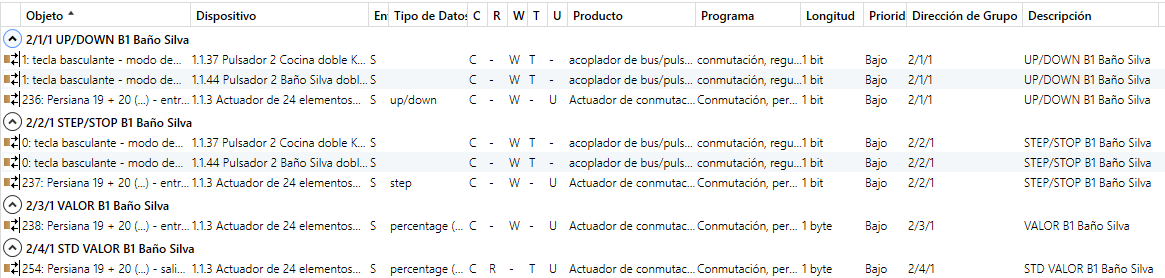
\includegraphics[width=1.15\textwidth]{figures/prog_pers.png}   
\caption{Programación genérica de la sección de Persianas}
\label{fig:prog_pers}
\end{figure}
\end{center}

\subsection{Climatización}Esta sección se trata de la que posee una mayor complejidad a la hora de programar debido a que debe integrar los numerosos módulos que la componen y por ello se ha creado el siguiente esquema simplificado para facilitar su comprensión:
 \begin{center}
\begin{figure}[H]
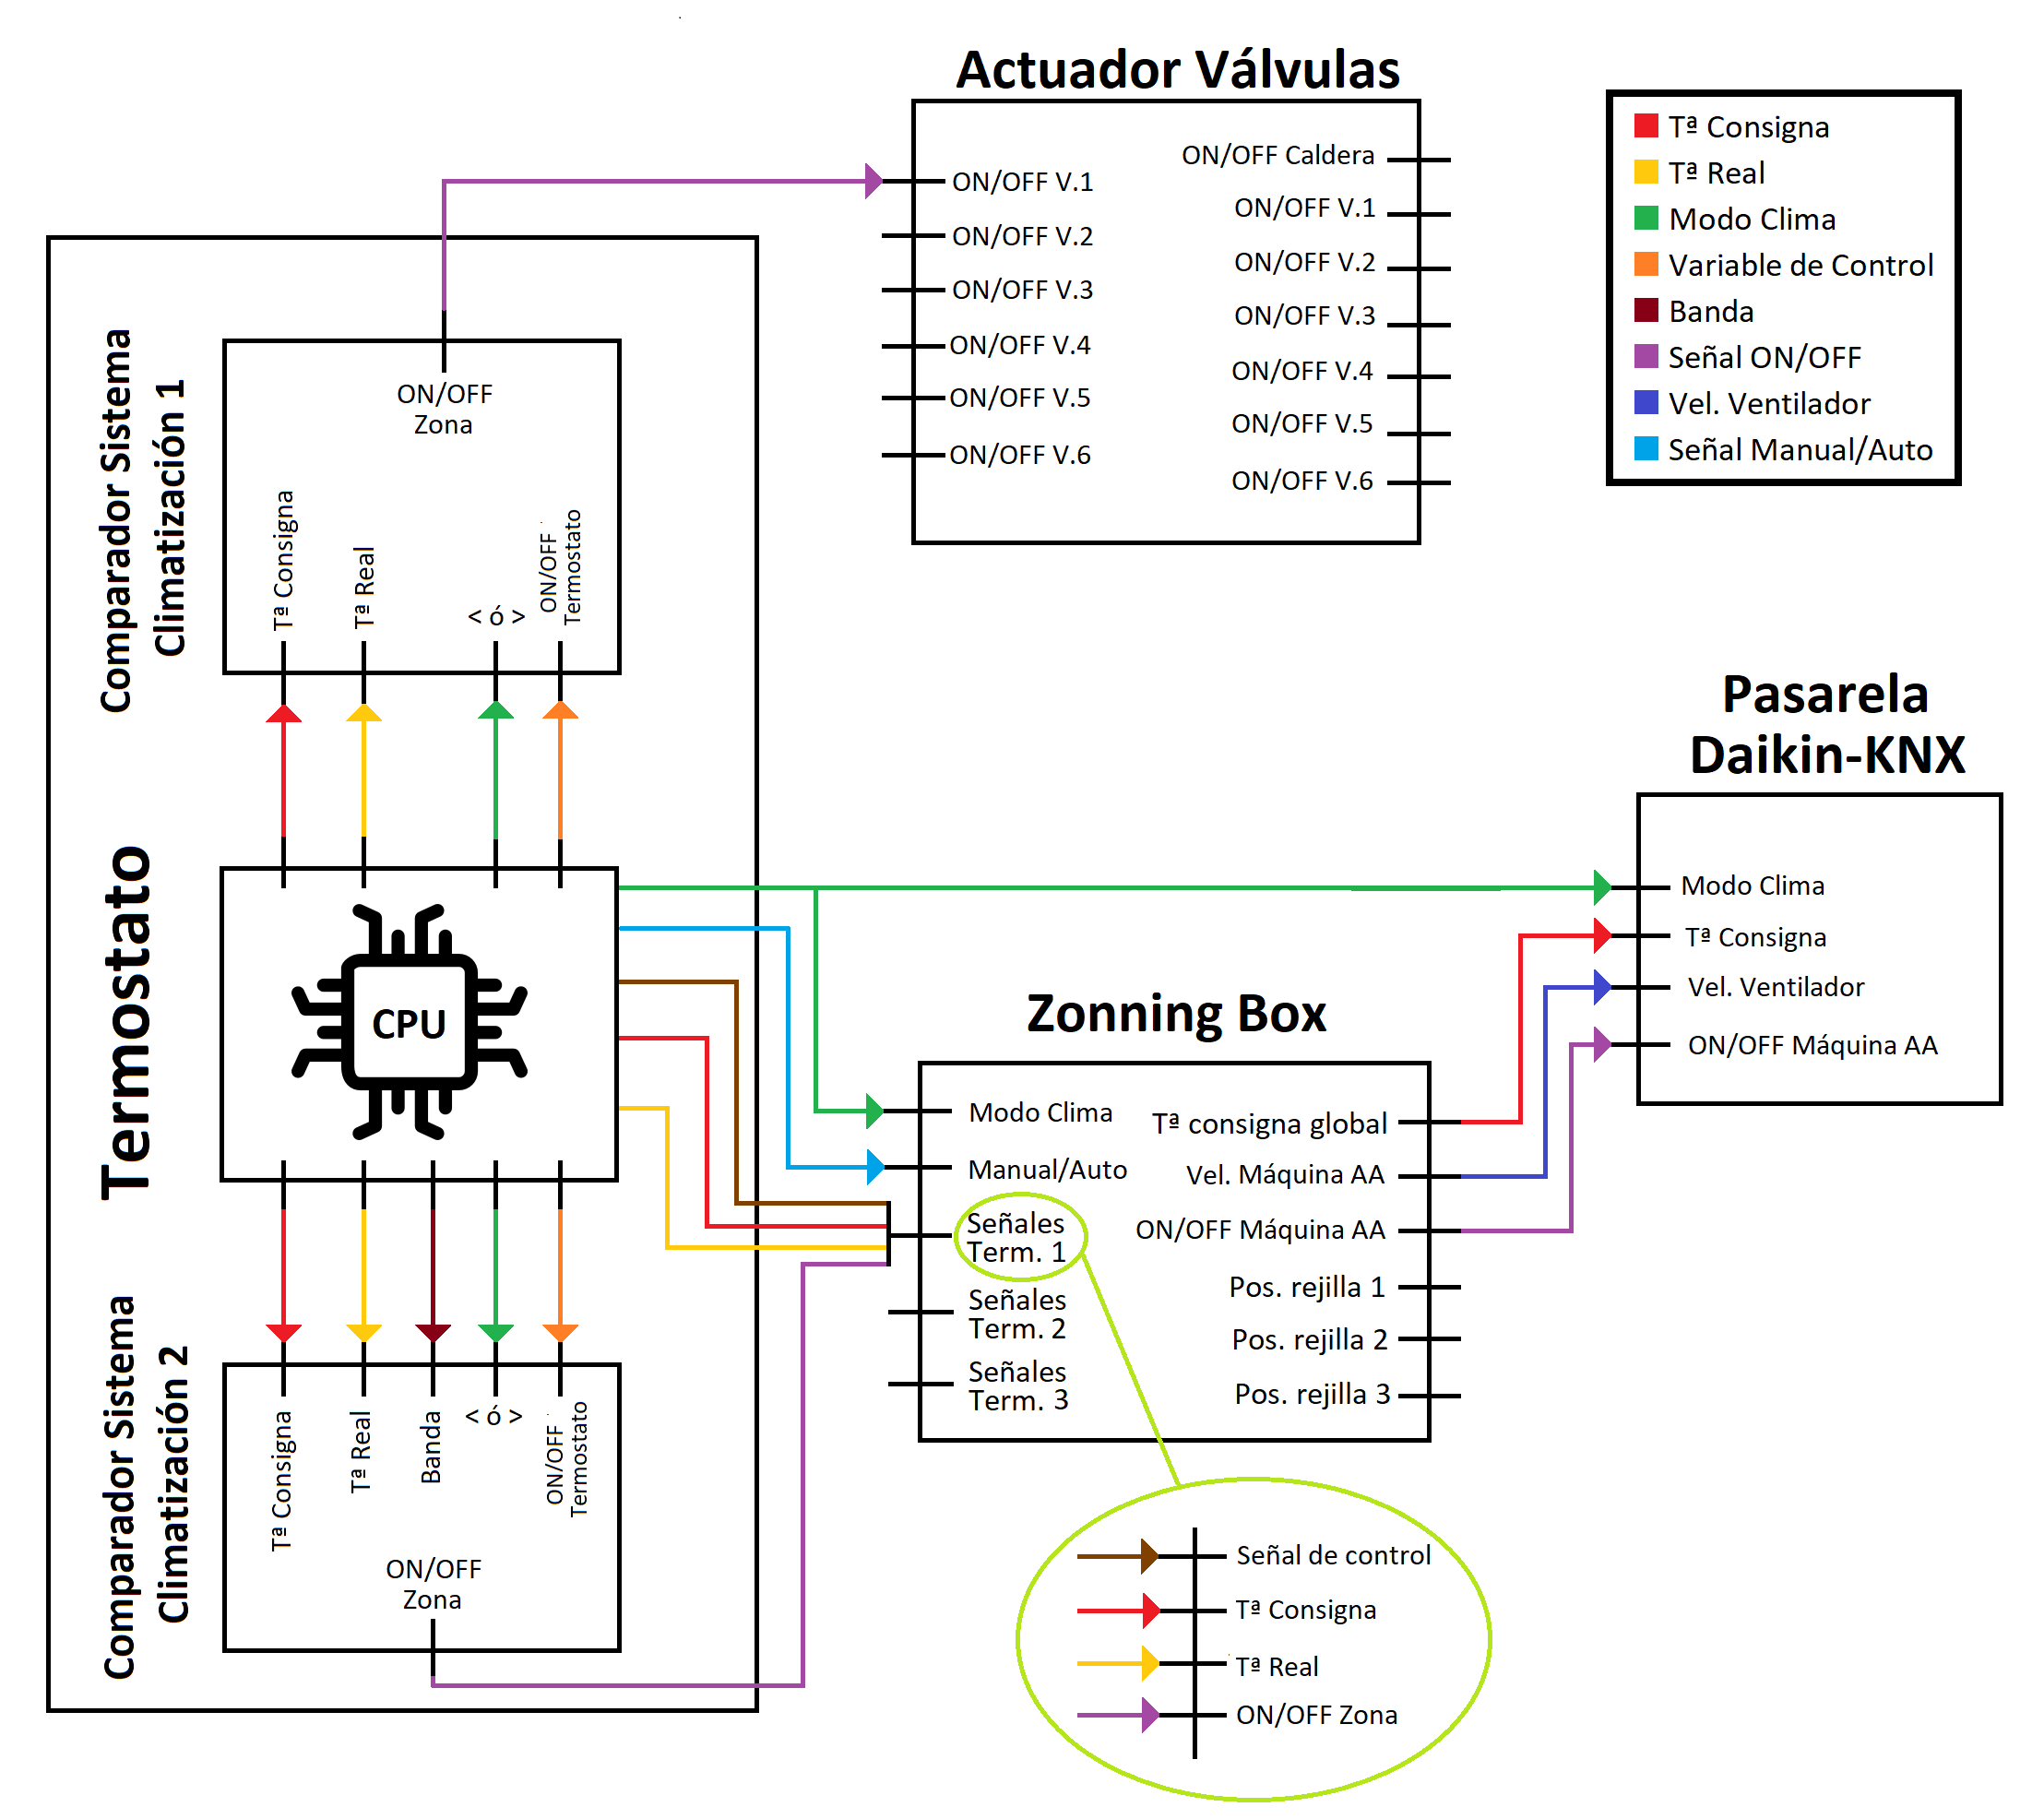
\includegraphics[width=1.15\textwidth]{figures/prog_termost.png}   
\caption{Esquema linkado sistema de climatización}
\label{fig:prog_termost}
\end{figure}
\end{center}
A la izquierda de la Imagen \ref{fig:prog_termost}, aparece uno de los termostatos a instalar en la vivienda. En su interior podemos encontrar su módulo de procesamiento, por el cual recibirá y retransmitirá todas las variables que componen el sistema de climatización enviadas desde la aplicación móvil, el X1 o desde sus propios pulsadores accionados por el cliente. \\Las variables que maneja serán las siguientes: 
\begin{itemize}
\item \textbf{Modo clima:} es el parámetro que indica al sistema si debe actuar controlando la temperatura de la vivienda en modo verano o generador de frio, o por el contrario, lo hará en modo invierno o generando calor. Tendrá un tamaño de 1 bit, asegurando así que el sistema no se encuentre en una situación de dualidad, pudiendo provocar errores o incluso el daño de los equipos de aerotermia. Será seleccionado por el usuario a través de la aplicación o del G1.
\item \textbf{Temperatura real:} será el valor medido de la temperatura de la habitación por el termómetro interno del termostato instalado en ella. Tendrá un tamaño de 2 bytes.
\item \textbf{Temperatura de consigna:} esta variable de 2 bytes reflejará el valor deseado por el cliente de temperatura en una determinada habitación y será seleccionada a través de los pulsadores de cada termostato o bien desde la aplicación o del G1. Como se explicó en la sección \ref{sec:sec_clima}, se ha optado por un control de tipo PI para lograr que la temperatura real logre igualarse a la de consigna.
\item \textbf{Banda:} este parámetro marcará la diferencia de temperatura requerida para que el sistema secundario de climatización comience a actuar en el modo de clima generador de calor. Es decir, si la banda tiene su valor fijado en 3ºC y la temperatura de consigna de la habitación es de 25ºC, la CPU no enviará una señal de encendido si la temperatura real se encuentra por encima de los 22ºC, de igual manera que si el sistema se encuentra muy por debajo de la consigna y pasado el rato supera el límite marcado por la banda, se enviará una señal de desconexión al sistema secundario de aerotermia. Al igual que las variables de temperatura, poseerá un tamaño de 2 bytes.
\item \textbf{Variable de control:} esta señal de 1 byte de tamaño será enviada a los controladores de los equipos de aerotermia indicando el porcentaje de apertura o demanda requerido por el sistema, en función de la magnitud de la diferencia entre las temperaturas real y de consigna de cada estancia.
\item \textbf{Señal de ON/OFF:} se trata de una señal tipo todo/nada, es decir, 1 bit,  que se enviará a los equipos en el momento en que haya demanda de calor o frio en las habitaciones y se cumplan los requisitos ya mencionados anteriormente.
\item \textbf{Modo manual/automático:} esta señal binaria (1bit), permitirá al usuario elegir entre el control manual o automático de los ventiladores del fancoil.
\item \textbf{Velocidad del ventilador:} esta señal, tal y como indica su nombre, marcará la velocidad a la que debe rotar el ventilador de la máquina de fancoil. Será enviada desde el módulo de actuación de rejillas si el usuario tiene seleccionado el modo automático, mientras que por el contrario, si se encuentra activado el modo manual, será el usuario a través de la aplicación o el G1 quien seleccione el nivel de velocidad deseado. Tendrá un tamaño de 1 byte.
\end{itemize}

\subsection{Sistemas sensoriales}
\subsection{Control de consumos}
\subsection{Escenas y centralizados}
\subsection{Sistemas de visualización y protocolo de comunicación}

\chapter{Pruebas y resultados}

En este capítulo del Trabajo se realizará un análisis de la fase final del proyecto, en la que, una vez finalizada la programación y la instalación de los dispositivos en la vivienda, se hará un examen exhaustivo al comportamiento de todos los mecanismos y la relación entre ellos,  comprobando la robustez del diseño y subsanando pequeños bugs o fallos no identificados en las fases anteriores, así como el funcionamiento adecuado de los equipos y mecanismos que lo componen.

\section{Puesta en marcha}
En esta sección se describirá en detalle la fase final del proyecto, consistente en que, una vez finalizada la instalación física de los componentes en la vivienda, se realizarán una serie de pruebas y comprobaciones para confirmar que tanto la programación como su volcado en los mecanismos han sido correctos, sin llegar a suceder o sin alcanzar algún estado inesperado o incorrecto que hiciese detenerse o incluso fallar el sistema completo. Con estas pruebas también se detectan fallos cometidos durante la fase de instalación del sistema eléctrico como cables mal etiquetados que dan lugar a confusiones y comportamientos anómalos de los mecanismos, o incluso derivaciones y otra serie de cuestiones relacionadas con el cableado y su acometida eléctrica. Todas estas pruebas, chequeos y correcciones se engloban en el término Puesta en Marcha.\\\\

Por motivos de tiempo, las primeras pruebas que se han realizado sobre los equipos son las relacionadas con los módulos lógicos implementados en el X1. Esto es debido a que en caso de no comportarse de manera idéntica en la instalación que en las simulaciones y pruebas en el ordenador, ya sea por contener programación incorrecta o por la influencia de otras variables del sistema no contempladas durante estas simulaciones, su modificación y posterior fase de pruebas y simulaciones tendría un gran coste en términos de tiempo, lo que finalmente se traduce en una pérdida del beneficio y del margen de ganancia que obtendría la empresa, alejándolo por tanto de su objetivo final.\\\\

Debido a este requerimiento de enviar a una persona a realizar pruebas sobre la propia instalación real, las simulaciones y pruebas en el ordenador toman una gran relevancia a la hora de no invertir o gastar recursos y tiempo que podrían restar valor final al total del proyecto. Por lo tanto, utilizando el software \textit{Gira Project Assistant}, se han testeado y comprobado encarecidamente las programaciones lógicas desarrolladas antes de realizar la prueba definitiva en la vivienda.\\\\

Una vez finalizada esta parte de la Puesta en Marcha, se continuará volcando la programación completa a todos los módulos y mecanismos que componen el sistema, permitiendo así realizar el resto de comprobaciones. Estas rutinas de chequeo han sido diseñadas y plasmadas en un documento (confidencial) por el propio ingeniero que ha diseñado el proyecto y posteriormente, ampliadas por expertos con mayor experiencia y conciencia de los fallos más habituales y también los más perjudiciales. Esta combinación permite buscar y encontrar con una mayor precisión y rapidez los errores cometidos a cualquier persona con cualificación y conocimientos en la materia, logrando así no copar el tiempo al completo del diseñador y programador. \\

Cuando todos los mecanismos hayan recibido su programación, se comenzará realizando las pruebas más simples, rápidas y sencillas como el ON/OFF de la las luminarias o la subida y bajada de las persianas, e irá incrementando su complejidad hasta finalmente realizar un chequeo completo del sistema de climatización teniendo en cuenta todas las posibilidades de combinaciones y comportamientos posibles que este sistema puede llegar a alcanzar. \\\\
Una vez se han validado todas las pruebas y especificaciones recogidas en el documento anteriormente mencionado, se realizará una demostración al cliente, explicando a su vez el funcionamiento final que tendrá el sistema instalado en su vivienda, validando de esta manera la consecución de los requisitos iniciales planteados y dando por finalizando así la Puesta en Marcha, y por tanto, el proyecto.


\section{Resultados}

Una vez expuestos las pruebas en la sección anterior, aquí se deben comentar y analizar su validez.

\section{Mejoras}

Una vez expuestos las pruebas en la sección anterior, aquí se deben comentar y analizar su validez.

\chapter{Gestión del proyecto}

En este capítulo se describe la gestión del proyecto: ciclo de vida, planificación, presupuesto, etc.

\section{Fases del proyecto}

Explicación de las fases del proyecto: definición, análisis, diseño, construcción, pruebas, implementación, validación, documentación. Ejemplo: diagrama de Pert.

\section{Metodología}
\subsection{Plan de trabajo}

\begin{itemize}
\item \textbf{T1. Fase de recursos}
	\begin{itemize}
	\item Obtención del software ETS5.
	\item Obtención del software Gira Project Assistant.
	\item Obtención de las especificaciones del proyecto.
	\item Obtención de bibliografía. \\
	\end{itemize} 
\item \textbf{T2. Análisis teórico previo}
	\begin{itemize}
	\item Estudio viabilidad y especificaciones del proyecto.
	\item Diseño de la solución.
	\item Ajustes y mediación con el cliente sobre las nuevas características o modificaciones del sistema.
	\item Elaboración del presupuesto.
	\item Elección y pedido del hardware en base a especificaciones finales. \\
	\end{itemize} 
\item \textbf{T3. Implementación en ETS5}
	\begin{itemize}
	\item Desarrollo de la arquitectura de la vivienda en el proyecto.
	\item Elaboración de los grupos de direcciones.
	\item Búsqueda y descarga de las bases de datos de los productos.
	\item Añadir los módulos de los dispositivos del sistema domótico.
	\item Asignar direcciones físicas a los dispositivos. \\
	\end{itemize} 
\item \textbf{T4. Análisis de desarrollo}
	\begin{itemize}
	\item Programación de parámetros de los dispositivos.
	\item Linkado de los objetos de comunicación de los dispositivos.
	\item Creación de escenas.
	\item Programación de módulos lógicos.
	\item Volcado de programación sobre los dispositivos físicos.
	\item Instalación de los dispositivos físicos en la vivienda. \\
	\end{itemize} 
\item \textbf{T5. Desarrollo sistema visualización}
	\begin{itemize}
	\item Creación servidor control remoto.
	\item Diseño y creación de las pantallas de visualización.
	\item Volcado sobre dispositivos físicos. \\
	\end{itemize} 
\item \textbf{T6. Validación y puesta en marcha del sistema}
	\begin{itemize}
	\item Comprobación instalación eléctrica y cableado.
	\item Testeo funcionalidades del sistema.
	\item Depuración de errores e implementación de mejoras. \\
	\end{itemize} 
\item \textbf{T7. Redacción de la memoria final} \\
\end{itemize} 

\subsection{Diagrama de Gantt}

\begin{table}[H]
\begin{ganttchart}[
canvas/.append style={fill=none, draw=black!5, line width=.75pt},
hgrid style/.style={draw=black!5, line width=1pt},
vgrid={*1{draw=black!5, line width=.75pt}},
x unit=1.2 cm,
y unit title=1 cm,
y unit chart=1 cm,
today label font=\small\bfseries,
title/.style={draw=none, fill=none},
title label font=\bfseries\footnotesize,
title label node/.append style={below=7pt},
include title in canvas=false,
bar label font=\mdseries\small\color{black!70},
bar label node/.append style={left=2cm},
bar/.append style={draw=none, fill=black!63},
bar incomplete/.append style={fill=green},
bar progress label font=\mdseries\footnotesize\color{black!70},
group incomplete/.append style={fill=blue},
group left shift=0,
group right shift=0,
group height=.5,
group peaks tip position=0,
group label node/.append style={left=.6cm},
group progress label font=\bfseries\small,
link/.style={-latex, line width=1.5pt, linkred},
link label font=\scriptsize\bfseries,
link label node/.append style={below left=-2pt and 0pt},
]{1}{10}
\gantttitle{Diagrama de Gantt}{10} \\[grid]
\gantttitle{Abril}{4}
\gantttitle{Mayo}{4}
\gantttitle{Junio}{2}\\
\gantttitle[title label node/.append style={below left=7pt and -3pt}]{Semana:\quad1}{1}
\gantttitlelist{2,...,10}{1} \\
\ganttbar[]{\textbf{T1}}{1}{1} \\
\ganttbar[]{\textbf{T2}}{2}{4} \\
\ganttbar[]{\textbf{T3}}{4}{4} \\
\ganttbar[]{\textbf{T4}}{5}{6} \\
\ganttbar[]{\textbf{T5}}{6}{6} \\
\ganttbar[]{\textbf{T6}}{7}{8} \\
\ganttbar[]{\textbf{T7}}{9}{10}
\end{ganttchart}
\caption{Diagrama de Gantt}
\label{tab:diagrama_gantt}
\end{table}



\section{Recursos}

\subsection{Personal}

Quien participa

\subsection{Material}

Quien lo proporciona

\subsection{Presupuesto}

En esta sección se realizará un recuento del precio y las unidades de los mecanismos adquiridos e instalados en la vivienda. Pese a que, tanto el beneficio económico como el tiempo de programación se vean perjudicados al adquirir los mecanismos a diferentes proveedores, es necesario la conjugación de varios de ellos para lograr cumplir con las expectativas del cliente en cuanto al alcance de la instalación. Por tanto, se detallará también la empresa que proporciona los módulos:

\newpage
\begin{flushleft}
\begin{longtable}[H]{|c|p{4cm}|c|c|c|c|}
\hline 
\rule[0mm]{0mm}{5mm}
\multirow{2}{*}{Referencia} &  \multirow{2}{*}{Descripción} & \multirow{2}{*}{ Fabricante} &  \multirow{2}{*}{Cantidad} & Precio  & Precio \\
&  &  &  &  Unitario &  Total\\
\hline
\hline
\endhead
\rule[0mm]{0mm}{4mm}
18327 & Base de enchufe 16A/250V & Gira &  & 6,44 & 0\\
\hline
\rule[0mm]{0mm}{4mm}
\multirow{2}{*}{25227} & Juego de juntas para  & \multirow{2}{*}{Gira} & \multirow{2}{*}{0} & \multirow{2}{*}{2,8} & \multirow{2}{*}{0}\\
 &  base de enchufe & & & &\\
\hline
\rule[0mm]{0mm}{4mm}
245200 & ? & Gira &  &  & 0\\
\hline
\rule[0mm]{0mm}{4mm}
27027 & ? & Gira &  &  & 0\\
\hline
\rule[0mm]{0mm}{4mm}
 \multirow{2}{*}{205127} & Detect. Movimiento  &  \multirow{2}{*}{Gira} &  \multirow{2}{*}{4} &  \multirow{2}{*}{169,67} &  \multirow{2}{*}{678,68}\\
 &  Komfort 2,2m KNX & & & &\\
\hline
\rule[0mm]{0mm}{4mm}
200800 & Acoplador de bus KNX & Gira & 6 & 51,29 & 307,74\\
\hline
\rule[0mm]{0mm}{4mm}
\multirow{2}{*}{222500} & Detect. Presencia  & \multirow{2}{*}{Gira} & \multirow{2}{*}{1} & \multirow{2}{*}{231,86} & \multirow{2}{*}{231,86}\\
 &  Mini Komfort KNX & & & &\\
\hline
\rule[0mm]{0mm}{4mm}
 \multirow{2}{*}{204127} & Detect. Movimiento &  \multirow{2}{*}{Gira} &  \multirow{2}{*}{1} &  \multirow{2}{*}{118,67} &  \multirow{2}{*}{118,67}\\
 &  Standard 2,2m KNX & & & &\\
\hline
\rule[0mm]{0mm}{4mm}
\rule[0mm]{0mm}{4mm}
\multirow{2}{*}{210427} & Sensor CO2 + & \multirow{2}{*}{Gira} & \multirow{2}{*}{1} & \multirow{2}{*}{336,58} & \multirow{2}{*}{336,58}\\
 &  Humedad KNX & & & &\\
\hline
\rule[0mm]{0mm}{4mm}
 \multirow{2}{*}{18200} & Pulsador KNX de 2 elem. &  \multirow{2}{*}{Gira} &  \multirow{2}{*}{37} &  \multirow{2}{*}{79,22} &  \multirow{2}{*}{2931,14}\\
 &  con mando de 1 punto & & & &\\
\hline
\rule[0mm]{0mm}{4mm}
29527 & Teclas basculantes & Gira & 35 & 4,85 & 169,75\\
\hline
\rule[0mm]{0mm}{4mm}
 \multirow{2}{*}{29427} & Teclas basculantes &  \multirow{2}{*}{Gira} &  \multirow{2}{*}{2} &  \multirow{2}{*}{6,66} &  \multirow{2}{*}{13,32}\\
 &  serigrafiadas con flecha & & & &\\
\hline
\rule[0mm]{0mm}{4mm}
\multirow{2}{*}{213000} & Fuente alimentacion& \multirow{2}{*}{Gira} & \multirow{2}{*}{1} & \multirow{2}{*}{323,37} & \multirow{2}{*}{323,37}\\
 &   640mA KNX  & & & &\\
\hline
\rule[0mm]{0mm}{4mm}
 \multirow{2}{*}{504000} & Actuador de conmutación &  \multirow{2}{*}{Gira} &  \multirow{2}{*}{2} &  \multirow{2}{*}{772,8} &  \multirow{2}{*}{1545,6}\\
 &  24 outs / 12 persianas 16A & & & &\\
\hline
\rule[0mm]{0mm}{4mm}
\multirow{2}{*}{212900} & Actuador calefaccion  & \multirow{2}{*}{Gira} & \multirow{2}{*}{2} & \multirow{2}{*}{231,83} & \multirow{2}{*}{463,66}\\
 & 6 elementos KNX & & & &\\
\hline
\rule[0mm]{0mm}{4mm}
 \multirow{2}{*}{212600} & Entrada binaria KNX de  &  \multirow{2}{*}{Gira} &  \multirow{2}{*}{4} &  \multirow{2}{*}{230,98} &  \multirow{2}{*}{923,92}\\
 & 6 elementos 10-230 V CA/CC & & & &\\
\hline
\rule[0mm]{0mm}{4mm}
 & Detector de humos & Gira &  &  & 0\\
\hline
\rule[0mm]{0mm}{4mm}
\multirow{2}{*}{234300} & Módulo KNX para  & \multirow{2}{*}{Gira} & \multirow{2}{*}{4} & \multirow{2}{*}{115,57} & \multirow{2}{*}{462,28}\\
 & detector de humo & & & &\\
\hline
\rule[0mm]{0mm}{4mm}
209600 & Gira X1 & Gira & 1 & 835,58 & 835,58\\
\hline
\rule[0mm]{0mm}{4mm}
206912 & Gira G1 & Gira & 1 & 1000,61 & 1000,61\\
\hline
\rule[0mm]{0mm}{4mm}
21122 & Marco cubierta 1 elemento & Gira &  & 3,3 & 0\\
\hline
\rule[0mm]{0mm}{4mm}
21222 & Marco cubierta 2 elemento & Gira &  & 4,54 & 0\\
\hline
\rule[0mm]{0mm}{4mm}
21322 & Marco cubierta 3 elemento & Gira &  & 8,3 & 0\\
\hline
\rule[0mm]{0mm}{4mm}
21422 & Marco cubierta 4 elemento & Gira &  & 13,4 & 0\\
\hline
\rule[0mm]{0mm}{4mm}
40000 & ? & Gira &  &  & 0\\
\hline
\rule[0mm]{0mm}{4mm}
27427 & ? & Gira &  &  & 0\\
\hline
\rule[0mm]{0mm}{4mm}
 \multirow{2}{*}{202500} & Actuador de regulacion KNX&  \multirow{2}{*}{Gira} &  \multirow{2}{*}{4} &  \multirow{2}{*}{529,2} &  \multirow{2}{*}{2116,8}\\
 & 4 elementos Komfort & & & &\\
\hline
\rule[0mm]{0mm}{4mm}
 \multirow{2}{*}{KCI 4 S0} & Interfaz KNX para  & \multirow{2}{*}{ Zennio} &  \multirow{2}{*}{2} &  \multirow{2}{*}{83,3} &  \multirow{2}{*}{166,6}\\
 & contadores de consumo & & & &\\
\hline
\rule[0mm]{0mm}{4mm}
\multirow{2}{*}{ZVI-F55D} & Panel táctil capacitivo  & \multirow{2}{*}{Zennio} & \multirow{2}{*}{6} & \multirow{2}{*}{116,2} & \multirow{2}{*}{697,2}\\
 & con display & & & &\\
\hline
\rule[0mm]{0mm}{4mm}
\multirow{2}{*}{ZCL-ZB4} &Actuador de clima con& \multirow{2}{*}{Zennio} &\multirow{2}{*}{2} & \multirow{2}{*}{125,3} & \multirow{2}{*}{250,6}\\
 & zonificación de 4 zonas & & & &\\
\hline
\rule[0mm]{0mm}{4mm}
\multirow{2}{*}{ZIO-KESP} & Medidor de energía & \multirow{2}{*}{Zennio} & \multirow{2}{*}{2} & \multirow{2}{*}{104,3} & \multirow{2}{*}{ 208,6}\\
 & eléctrica KNX KES Plus  & & & &\\
\hline
\rule[0mm]{0mm}{4mm}
{\small ZN1AC-CST120} & Transformador de corriente & Zennio & 6 & 16,8 & 100,8\\
\hline
\hline
\rule[0mm]{0mm}{4mm}
 & & & &TOTAL&12.459,56 €\\
\hline 
\caption{Presupuesto materiales}
\label{tab:tabla_presupuesto_mat}
\end{longtable}
\end{flushleft}

\begin{center}
\begin{longtable}[H]{|c|c|c|c|c|c|}
\hline 
\rule[0mm]{0mm}{5mm}
\multirow{2}{*}{Descripción} & \multirow{2}{*}{ Empresa} &  \multirow{2}{*}{Cantidad} & Precio  & \multirow{2}{*}{Tiempo} & Precio \\
&  &  &  Unitario &  & Total\\
\hline
\hline
\endhead
\rule[0mm]{0mm}{4mm}
Instalador & Freedom & 2 & 878,63 &  2 meses & 3514.4\\
\hline
\rule[0mm]{0mm}{4mm}
Ingeniero & Freedom & 1 & 1.712,42 & 2 meses & 3424,84\\
\hline
Licencia & KNX & 1 & 1000 & - & 1000\\
\hline
Material & Varios & 1 & 12,459,56 & - & 12,459,56\\
\hline
\hline
\rule[0mm]{0mm}{4mm}
 & & & &TOTAL&20398.80 €\\
\hline 
\caption{Presupuesto}
\label{tab:tabla_presupuesto}
\end{longtable}
\end{center}

\chapter{Conclusiones}

\section{Conclusiones}

Tras la realización completa de este proyecto, pasando por todas las fases de su desarrollo: desde su diseño hasta su implementación y puesta en marcha, pasando por el estudio de los materiales y componentes a instalar, se han obtenido una serie de conclusiones que a continuación se pasan a detallar. \\\\
En primer lugar, se ha determinado que una buena organización permite el desarrollo óptimo del proceso, tanto en la cuestión temporal como económica, ya que al encontrarse planificada cada una de estas fases y conociendo los materiales que van a ser necesarios en cada una de ellas, se podrá disponer del personal necesario en cada momento para la consecución de los objetivos marcados, sin ser penalizados con cualquier desavenencia causada por estos mismos motivos. En este aspecto también se destacan las facilidades que otorga el ser poseedor de los contactos necesarios de los proveedores de material, para lograr los precios más bajos y las menores demoras posibles en la entrega del material.\\
Por otro lado, también favorece el desarrollo adecuado el conocer de primera mano los requisitos exigidos para la creación del sistema, así como las peculiaridades que se van a encontrar a la hora de su programación e instalación en la vivienda, como puede ser el espacio y otras capacidades físicas de la vivienda.\\
Otra conclusión obtenida del desarrollo de este proyecto es que, como se pude observar en el caso de la programación de las luminarias tipo Dimmer, es que las simulaciones realizadas en un ordenador siempre funcionarán de manera correcta, pero esto no implica que al volcar esa programación en los módulos reales, el sistema vaya a comportarse de la misma manera que lo hacía en las pruebas virtuales, por lo que se ha de tener muy presente y dar una gran importancia a la fase de pruebas y puesta en marcha.\\\\
Finalmente, el cliente quedo satisfecho con el resultado de la instalación, por lo que como conclusión final destacaría la importancia de contar con un equipo cualificado y con experiencia en el sector que se encargue rápidamente de cualquier problema o desavenencia que pueda aparecer con el proceso, así como la fluidez en la comunicación con el propio cliente.


\section{Futuras líneas de trabajo y aplicación}

Como se ha venido comentando a lo largo de todo el documento, esta tecnología se encuentra ahora mismo en plena ola de desarrollo y mejora, por lo que en los próximos años es muy probable que se desarrollen y se saquen al mercado módulos con funcionalidades totalmente innovadoras que permitan  llevar la domótica y la inmótica al siguiente nivel: la domotización de una ciudad completa. Esta futurística idea, podría permitir controlar y gestionar una ciudad entera desde un ordenador, pudiendo llegar a lograr reducir y optimizar el uso de la energía en una amplia región densamente poblada a la vez que se realizan otro tipo de gestiones para mejorar el confort y la vida en la ciudad, como por ejemplo, la gestión de atascos, el control de la iluminación pública o la emisión de gases contaminantes, entre muchos otros. Algo más cercano, y que ya comienza a darse en la realidad, es la domotización de los grandes edificios de nueva construcción, acercándose así a la idea del control de todos los edificios de una región  y aplicando notables mejoras en la eficiencia energética y el consumo. \\\\
Por otro lado, y con los nuevos avances tecnológicos, es bastante probable que la domótica alcance al sector de la Salud, y comiencen a desarrollarse mecanismos y módulos que permitan a los pacientes de hospitales o personas con necesidades especiales tener una vida más cómoda y  sencilla en lo que respecta a la realización de tareas no complejas que se realizan a diario, como su desplazamiento por interiores, hacer la compra o darse una ducha.\\\\
Concretamente para este proyecto, una de las futuras líneas de trabajo que se generan, es aquella que se comentó al comienzo del documento, que hablaba acerca de la modularidad del sistema y la capacidad de que la vivienda pueda ser dividida en dos en un futuro. Esta mejora precisaría de poco trabajo, ya que, con esta perspectiva, el ingeniero decidió preparar todo el sistema para que esta transición fuese lo menos laboriosa posible, aprovechando el tener fresco todo el sistema y el conocimiento absoluto de su funcionamiento, dos factores importantes de cara a que esta modificación sea realizada en un espacio de tiempo largo o bien, sea otra persona completamente diferente el que se encargue de implementarla. De este aspecto también se obtiene como conclusión que, haciendo uso de una buena documentación y el uso de nombres genéricos y muy concisos, cualquier persona puede integrarse de manera relativamente sencilla en el desarrollo o mejora de esta instalación.


\appendix

\chapter{Anexo: Documentación de la librería Travis}

{\Large Se muestra a continuación la documentación del código de la librería Travis, realizada con un generador de documentación automático. En nuestro caso, el documentador elegido es Doxygen.}


\appendix

\chapter{appendix}

En este apéndice...


\section{Lorem ipsum}
Lorem ipsum dolor sit amet, consectetur adipiscing elit. Maecenas ornare erat nisl, a laoreet purus pellentesque id. Duis laoreet ipsum posuere est hendrerit, quis ornare nisi iaculis. Quisque imperdiet gravida egestas. Maecenas in mauris felis. Quisque quis imperdiet enim. Curabitur dignissim eget nisi lobortis placerat. Donec et magna rutrum, tempor magna a, consectetur tortor. Donec faucibus sodales sem, eu iaculis leo eleifend id. Nam semper lectus nisl, sed molestie erat pharetra quis. Quisque vestibulum metus elit, id interdum ligula dignissim a.

Praesent eu velit ac lectus tristique tristique vitae et tellus. Mauris dignissim feugiat orci, vitae luctus dolor finibus ut. Ut congue bibendum lectus, vitae congue ligula. Donec commodo, lacus ac iaculis scelerisque, nunc purus finibus diam, at lacinia sem justo non quam. Aenean tempor urna vitae quam pretium porta. Sed in lacinia ipsum. Class aptent taciti sociosqu ad litora torquent per conubia nostra, per inceptos himenaeos. Integer ut tristique est. Nam vitae interdum ligula, ac sodales dolor. Nulla mollis bibendum urna, sit amet interdum est aliquet at. Sed sagittis mi vel tellus posuere, eu rutrum arcu tristique.

Vestibulum aliquet orci pharetra justo auctor, pharetra viverra felis finibus. Ut ac gravida quam. Donec egestas turpis nisi, nec elementum orci feugiat at. In hac habitasse platea dictumst. Praesent mollis sem in felis feugiat, dapibus finibus metus scelerisque. Aliquam ultricies ante quis nibh laoreet, ac aliquam justo maximus. Etiam rhoncus pharetra imperdiet.

Nullam at libero quis augue tristique luctus eget placerat lorem. Donec pretium, dui scelerisque dapibus feugiat, ex lacus auctor ipsum, in ultricies odio justo in eros. Proin sodales velit non accumsan tempor. Mauris at consectetur est. Donec aliquam porttitor tortor, id malesuada nunc euismod vel. Ut id ullamcorper turpis, nec feugiat sapien. Lorem ipsum dolor sit amet, consectetur adipiscing elit. Morbi aliquam tempus tortor, et gravida lectus iaculis non. Interdum et malesuada fames ac ante ipsum primis in faucibus. Pellentesque habitant morbi tristique senectus et netus et malesuada fames ac turpis egestas. Integer non maximus felis. Nullam ac tempor augue. Vestibulum in efficitur mauris. Sed in nulla ultrices, pharetra ligula et, blandit nunc. Quisque dictum magna eget diam maximus, ac pulvinar nisi tempor. Pellentesque quis feugiat elit.

Integer euismod in urna id placerat. Etiam urna elit, tempor et turpis venenatis, volutpat viverra lacus. In luctus arcu sit amet lectus rutrum, id ultricies mi pellentesque. Nulla bibendum, orci in elementum aliquam, mi purus sollicitudin orci, quis ornare nulla arcu placerat urna. Integer consequat, risus ac elementum pellentesque, nulla est lobortis justo, sed mattis nibh ligula nec velit. Integer sem mauris, luctus vitae venenatis a, tincidunt egestas purus. In et lectus semper, dapibus massa sed, ultrices nisi. Ut sit amet dolor porta, accumsan lectus ut, semper tellus. Praesent velit odio, facilisis quis sodales vel, molestie at risus. In sollicitudin mauris risus, ullamcorper ullamcorper ligula commodo sed. Ut libero tortor, rhoncus ut sagittis quis, fringilla nec nunc. Ut efficitur nisi id leo feugiat ultrices. Class aptent taciti sociosqu ad litora torquent per conubia nostra, per inceptos himenaeos. Sed at malesuada arcu.

Cum sociis natoque penatibus et magnis dis parturient montes, nascetur ridiculus mus. Sed consectetur, justo nec scelerisque accumsan, leo erat dictum odio, id feugiat nibh felis vel ipsum. Duis urna ante, commodo vitae neque varius, congue egestas turpis. Donec condimentum ullamcorper dapibus. Nulla sed sapien eu diam commodo finibus. Nulla fringilla lectus vitae augue rutrum volutpat. Nulla in accumsan orci. Suspendisse eget diam massa.

\backmatter
%Glosario, lista de símbolos, notas, etc.

%estilo de bibliografía: plana, alfa...
\bibliographystyle{plain}

%genera doble hoja en blanco
\cleardoublepage

%apartado de bibliografía
\addcontentsline{toc}{chapter}{Bibliography}

%se incluye la bibliografía. Archivo de tipo .bib (bibtex)
\bibliography{bibliography/bibliografia}

%fin del documento
\end{document}